\RequirePackage{lmodern}
  \DeclareFontFamily{OT1}{phv}{}\DeclareFontFamily{T1}{phv}{}
  \DeclareFontShape{OT1}{phv}{m}{n}{<->ssub*lmss/m/n}{}\DeclareFontShape{T1}{phv}{m}{n}{<->ssub*lmss/m/n}{}
  \DeclareFontShape{OT1}{phv}{b}{n}{<->ssub*lmss/bx/n}{}\DeclareFontShape{T1}{phv}{b}{n}{<->ssub*lmss/bx/n}{}
  \DeclareFontShape{OT1}{phv}{bx}{n}{<->ssub*lmss/bx/n}{}\DeclareFontShape{T1}{phv}{bx}{n}{<->ssub*lmss/bx/n}{}
  \DeclareFontFamily{OT1}{pcr}{}\DeclareFontFamily{T1}{pcr}{}
  \DeclareFontShape{OT1}{pcr}{m}{n}{<->ssub*lmtt/m/n}{}\DeclareFontShape{T1}{pcr}{m}{n}{<->ssub*lmtt/m/n}{}
\documentclass[journal,a4paper]{IEEEtran}

\usepackage[T1]{fontenc}
\usepackage{microtype}
\usepackage{graphicx}
\usepackage{booktabs}
\usepackage{tabularx}
\usepackage{array}
\usepackage{multirow}
\usepackage[table]{xcolor}
\usepackage{enumitem}
\usepackage{amsmath}
\usepackage{ragged2e}
\usepackage[numbers,sort&compress]{natbib}
\usepackage{xurl}
\usepackage[hidelinks]{hyperref}
\hypersetup{pdftitle={Where the Flood Reached: Terrain-Only Classical Machine Learning of Building Damage in the 2026 Langtang Lirung-Trishuli Debris Flood, Nepal},pdfauthor={Rustam Niraula},pdfkeywords={building damage, debris flood, HAND, spatial cross-validation, transferability, Nepal, Langtang, Trishuli},pdfsubject={Terrain-only machine learning of building damage}}

\setlist{itemsep=1pt,topsep=3pt}
\renewcommand{\topfraction}{0.9}
\renewcommand{\dbltopfraction}{0.9}
\renewcommand{\bottomfraction}{0.8}
\renewcommand{\textfraction}{0.07}
\renewcommand{\floatpagefraction}{0.8}
\renewcommand{\dblfloatpagefraction}{0.8}
\newcolumntype{L}[1]{>{\RaggedRight\arraybackslash}p{#1}}
\newcolumntype{Y}{>{\RaggedRight\arraybackslash}X}

\begin{document}

\title{Where the Flood Reached: Terrain-Only Classical Machine Learning of Building Damage in the 2026 Langtang Lirung--Trishuli Debris Flood, Nepal}

\author{\IEEEauthorblockN{Rustam Niraula}\\[3pt]
\IEEEauthorblockA{\textit{MSc. Data Science and Computational Intelligence} \\
\textit{Softwarica College of IT and E-commerce (Coventry University)}\\
260119@softwarica.edu.np}
}

\markboth{Niraula: Terrain-only machine learning of building damage, Trishuli 2026}{Niraula: Terrain-only ML of building damage, Trishuli 2026}

\maketitle

\begin{abstract}
On 26 August 2026 a rock--ice avalanche from Langtang Lirung (7,227\,m) became a debris flood that ran more than 90\,km down the Bhote Koshi--Trishuli valley, Nepal. We ask whether terrain alone, from a 30\,m elevation model, can predict which buildings were damaged, and how well such a model transfers to a part of the valley it has not seen. Copernicus EMSR927 damage grades were joined to pre-event Overture footprints: 17,503 buildings (3,360 affected, 2,505 destroyed) in three reaches. Ten terrain features were used with nine classical learners, each tested on a reach left out of training. Over all buildings, class-weighted logistic regression transferred best (held-out ROC-AUC 0.95--0.98), but most of that score comes from hillside buildings that no flood could reach. Among the near-channel buildings, within 30\,m height and 300\,m distance of the flood path, terrain still ranks affected buildings in an unseen reach with AUC 0.80--0.85 and destroyed buildings with 0.78--0.86. There, height above the flood path (HAND) alone ranks as well as the full model; what the model adds is a probability and a data-derived decision threshold. Flexible learners failed outside their training terrain. The height above the river at which damage becomes likely fell by about 20\,m per doubling of distance from the source, from about 87\,m near the border to 16\,m at 90\,km ($R^2 = 0.94$). The ranking transferred between reaches but the probability level did not: the upstream reach was under-predicted and the downstream reach over-predicted. Re-fitting only the intercept on 20--50 labelled buildings removed most of this error. Terrain gives a transferable ranking of exposure; the probability level, and therefore the decision threshold, must come from the event.
\end{abstract}

\begin{IEEEkeywords}
debris flood; building damage; Height Above Nearest Drainage; logistic regression; spatial transfer; calibration; area of applicability; Nepal Himalaya.
\end{IEEEkeywords}

\section{Introduction}\label{sec:intro}

At 08:37 local time on 26 August 2026, a rock--ice mass on the north face of Langtang Lirung failed at about 5,100--5,200\,m, fell into the Lhende Khola valley and became a debris flood along the Bhote Koshi and Trishuli rivers \citep{icimod2026}. Within an hour it destroyed the Rasuwagadhi border crossing, damaged several hydropower plants and struck settlements from Timure to Betrawati and beyond \citep{icimod2026,li2026}. Events of this kind recur across High Mountain Asia: an inventory of High Mountain Asia lists 60 large rock and ice avalanches, 29 of which cascaded into floods or debris flows \citep{zhong2024}, and the 2023 South Lhonak outburst in Sikkim showed how a single high-mountain failure can damage infrastructure a hundred kilometres downstream \citep{sattar2025}.

\paragraph{What is known} Studies of Himalayan cascades reconstruct the physical event and count what was exposed. They overlay modelled or mapped flood extents on buildings, roads and hydropower \citep{sattar2025,gouli2025,chen2025,li2026}, or survey losses after the event \citep{duwadi2024}. Building-level damage models exist for floods and debris flows elsewhere, but they rely on simulated or surveyed flow depth, velocity and impact pressure \citep{paulik2023,wuthrich2024,barnhart2024,wang2026}. Machine-learning damage models for Nepal exist only for earthquakes, where structural survey data are available \citep{ghimire2022}. Table~\ref{tab:lit} compares these studies.

\paragraph{How they are tested} Three weaknesses recur in how these models are evaluated. First, many are fitted and scored on the same buildings: the vulnerability curves of \citet{wang2026} reach an accuracy above 85\% on the 36 buildings they were fitted to, and \citet{barnhart2024} test forecasts on the single event that motivated them. Second, where machine learning is used, train and test buildings are often drawn at random from the same area, so neighbours that share terrain and flood exposure end up on both sides of the split; \citet{currie2026} show that skill falls from a median macro-F1 of 0.68 to 0.54 once whole events are held out. Third, damage is rare, and accuracy or uncorrected scores on imbalanced data can look good while missing most damaged buildings \citep{elreedy2023,vandengoorbergh2022}. Flood susceptibility studies in Nepal use the same conditioning factors as this study (wetness index, stream power, distance to river) but map land, not buildings \citep{duwal2023}. A model that is to be used on a new valley needs to be tested on a place it has not seen, with metrics that do not hide the minority class.

\paragraph{Why terrain} For a cascade like this one, terrain is the only input that is known everywhere, in advance and at the scale of single buildings. Rainfall, lake levels and slope movement say whether and when a flood may start, but not which houses it will reach. Height Above Nearest Drainage turns an elevation model into the vertical distance a flood must rise to reach each point, and it underlies the national flood-inundation mapping of the United States, where it is combined with rating curves to convert a discharge into a flooded extent \citep{aristizabal2024}. In a steep Himalayan valley, a debris flood is confined between valley walls, so the height a building sits above the river should matter even more than on a lowland floodplain. What is not known is how well such terrain proxies predict actual building damage, and how the critical height changes as the flood loses energy downstream.

\paragraph{The gap} Four gaps follow from Table~\ref{tab:lit}.
(i) None of the Himalayan cascade studies reviewed here learns from \emph{observed} building damage; they count exposure, and none predicts damage.
(ii) Damage models need hydraulic intensities that do not exist for a fast, unmonitored cascade; whether terrain-only proxies such as Height Above Nearest Drainage (HAND; \citealp{aristizabal2024}) can stand in is untested.
(iii) Damage models lose accuracy when moved to new places \citep{paulik2023,currie2026}, and \citet{ghimire2023} name this host-to-target transfer as an open problem. Along a single cascade the flood weakens downstream, so the loss should be systematic and measurable.
(iv) Event size controls how many buildings are damaged \citep{barnhart2024}, yet a terrain-only model knows nothing about event size. How such a model should be generalised has not been examined.

\paragraph{Aim and research questions} We build and evaluate terrain-only models of observed building damage for the 2026 cascade with transparent, classical machine learning, and measure how they transfer along the valley. The questions are:
\begin{enumerate}[label=\textbf{RQ\arabic*.},leftmargin=2.6em]
  \item How well do pre-event terrain features predict whether a building was \emph{affected}, whether it was \emph{destroyed}, and, among affected buildings, whether it was destroyed rather than damaged?
  \item How does the height above the river at which damage becomes likely (HAND$_{50}$) change with distance downstream?
  \item Which classical learners transfer best to an unseen reach, and why?
  \item What transfers to a new reach, or a new flood: the ranking of buildings, the probabilities, or both?
\end{enumerate}

\paragraph{Contributions} (1) To our knowledge, the first classical machine-learning model of observed building damage for a Himalayan rock--ice debris-flood cascade, evaluated on an unseen reach both over all buildings and, as the headline measure, over the near-channel buildings where the flood-extent signal is removed. (2) A quantified attenuation curve of the damaging height above the river. (3) A transfer test along one cascade, with an explanation of why flexible models fail. (4) A separation of what transfers (the ranking) from what does not (the probability level, and with it the decision threshold), with a cheap way to recalibrate.

\paragraph{Definitions} \emph{Affected} means any Copernicus grade (destroyed, damaged or possibly damaged). \emph{Reach} is one of three river sections (upper, middle, lower; Section~\ref{sec:data}). \emph{Transfer} means training on two reaches and testing on the third. \emph{HAND} is the height of a building above the nearest cell of the traced flood path.

Section~\ref{sec:data} describes the study area and data, Section~\ref{sec:methods} the methods, Section~\ref{sec:results} the results, Section~\ref{sec:discussion} the discussion and Section~\ref{sec:conclusion} the conclusions.

\begin{table*}[tp]
\centering\footnotesize
\setlength{\tabcolsep}{3pt}
\caption{Comparison of related studies. Performance is given where the paper reports a single figure; ``--'' means the study is descriptive or reports no comparable figure.}\label{tab:lit}
\begin{tabularx}{\textwidth}{@{}L{2.3cm}L{2.2cm}L{3.6cm}L{2.7cm}L{2.6cm}Y@{}}
\toprule
\textbf{Author (year)} & \textbf{Hazard / region} & \textbf{Feature extraction} & \textbf{Model} & \textbf{Performance} & \textbf{Limitations}\\
\midrule
\citet{paulik2023} & Floods (6 events) & Up to 7 hazard and building variables, observed depth & Random forest regression; spatial transfer test & Precision falls when transferred between flood types & Needs observed depth; building attributes\\
\citet{wuthrich2024} & Flash flood, Germany & Field-surveyed depth, velocity, distance to bank, construction & Statistical analysis & -- & Not predictive\\
\citet{barnhart2024} & Debris flow, USA & Simulated depth, momentum flux (3 runout models) & Fragility functions & Best forecast: hit rate 48\%, threat score 25\% & Needs runout model and event volume; one event, no transfer test\\
\citet{wang2026} & Debris flow, SW China & FLO-2D depth, velocity, impact pressure; field survey & Lognormal vulnerability curves (vs.\ 4 other forms) & Prediction accuracy $>$85\% (in-sample fit) & 36 damaged buildings, one village; no held-out test\\
\citet{ghimire2022} & Earthquake, Nepal & Structural parameters + ShakeMap intensity & LR, SVR, RF, GB & 68\% accuracy (3 classes); 64\% with 4 features & Needs structural survey\\
\citet{ghimire2023} & Earthquake, Italy & Age, storeys, area, height + intensity & RF, GB, XGBoost & 72\% (all) / 68\% (basic) accuracy & Needs structural data; transfer untested\\
\citet{currie2026} & 11 disasters, global; floods excluded & Sentinel-1 coherence, intensity and texture & Random forest; leave-one-event-out & Median macro-F1 68\% $\rightarrow$ 54\% on unseen events & Needs post-event imagery; uncalibrated scores\\
\citet{duwal2023} & Riverine flood, Nepal & 10 conditioning factors incl.\ TWI, SPI, distance to river & SVM, RF, ANN & SVM best by AUROC & Land, not buildings\\
\citet{sattar2025} & Outburst cascade, India & Remote sensing, hydrodynamic modelling & Physical reconstruction & -- & Impacts counted, not predicted\\
\citet{zhong2024} & Rock--ice avalanches, HMA & Event inventory (60 events) & Inventory statistics & -- & Event level; no building impacts\\
\citet{gouli2025} & Outburst floods, China--Nepal & Lake and terrain factors & ML susceptibility + hydrodynamic model & -- & Exposure, not damage\\
\citet{chen2025} & Outburst floods, Nepal & Multi-temporal imagery & RF, Bayesian regression, flood model & -- & Exposure only\\
\citet{li2026} & \textbf{This event} & Precipitation, temperature, UNOSAT damage & Exposure overlay & -- & No predictive model\\
\midrule
\textbf{This study} & \textbf{This event} & 10 terrain features from a 30\,m DEM & 9 classical learners; leave-one-reach-out & AUC 95.8--98.3\% (affected, unseen reach); 80--85\% within 300\,m of the flood path & Single event; photo-interpreted labels; part of the skill is flood extent\\
\bottomrule
\end{tabularx}
\end{table*}

\section{Study area and data}\label{sec:data}

\subsection{Study area}
The study covers the Bhote Koshi--Trishuli corridor in Rasuwa and Nuwakot districts, from the border at Rasuwagadhi to the end of the Phosretar mapping area, 91\,km downstream along the flood path (Fig.~\ref{fig:map}). The upper part is a steep, narrow gorge; below Betrawati the valley widens and the channel flattens. The four Copernicus mapping areas form three reaches (Table~\ref{tab:reaches}). The Copernicus mapping areas leave a gap between about 16 and 42\,km, so no analysed buildings lie there.

The reaches differ in setting as much as in distance. The upper reach (Syaprubesi and Timure) lies in a gorge: the channel falls 2.2--2.9\% (interquartile range at the buildings) and the valley floor within 20\,m of the river is 130--155\,m wide; settlements sit on terraces and fans tens of metres above the river. In the middle reach (Betrawati--Bidur) the channel slope drops to 0.5--1.0\% and the valley floor widens to 190--260\,m, with dense settlement on low terraces close to the channel. The lower reach (Phosretar) is flatter still (0.2--0.4\%) and wider (210--390\,m), with scattered buildings on both banks. The share of buildings affected falls from 77\% upstream to 9\% downstream (Table~\ref{tab:reaches}), which already shows how the flood weakened with distance.

The event itself was poorly observed. There were no instruments above 5,500\,m at the source, the first hydrological confirmation came about 28 minutes after the seismic signal of the collapse, and SMS alerts were sent at 09:15--09:16, about 15 minutes after Timure had been flooded \citep{icimod2026}. The Galchhi gauge, about 100\,km downstream, recorded a 9\,m rise in 30 minutes. No flow depths, velocities or deposit thicknesses exist for the settlements, which is why the hydraulic inputs of physically based damage models \citep{barnhart2024,wang2026} are not available here.

\begin{figure}[t]
  \centering
  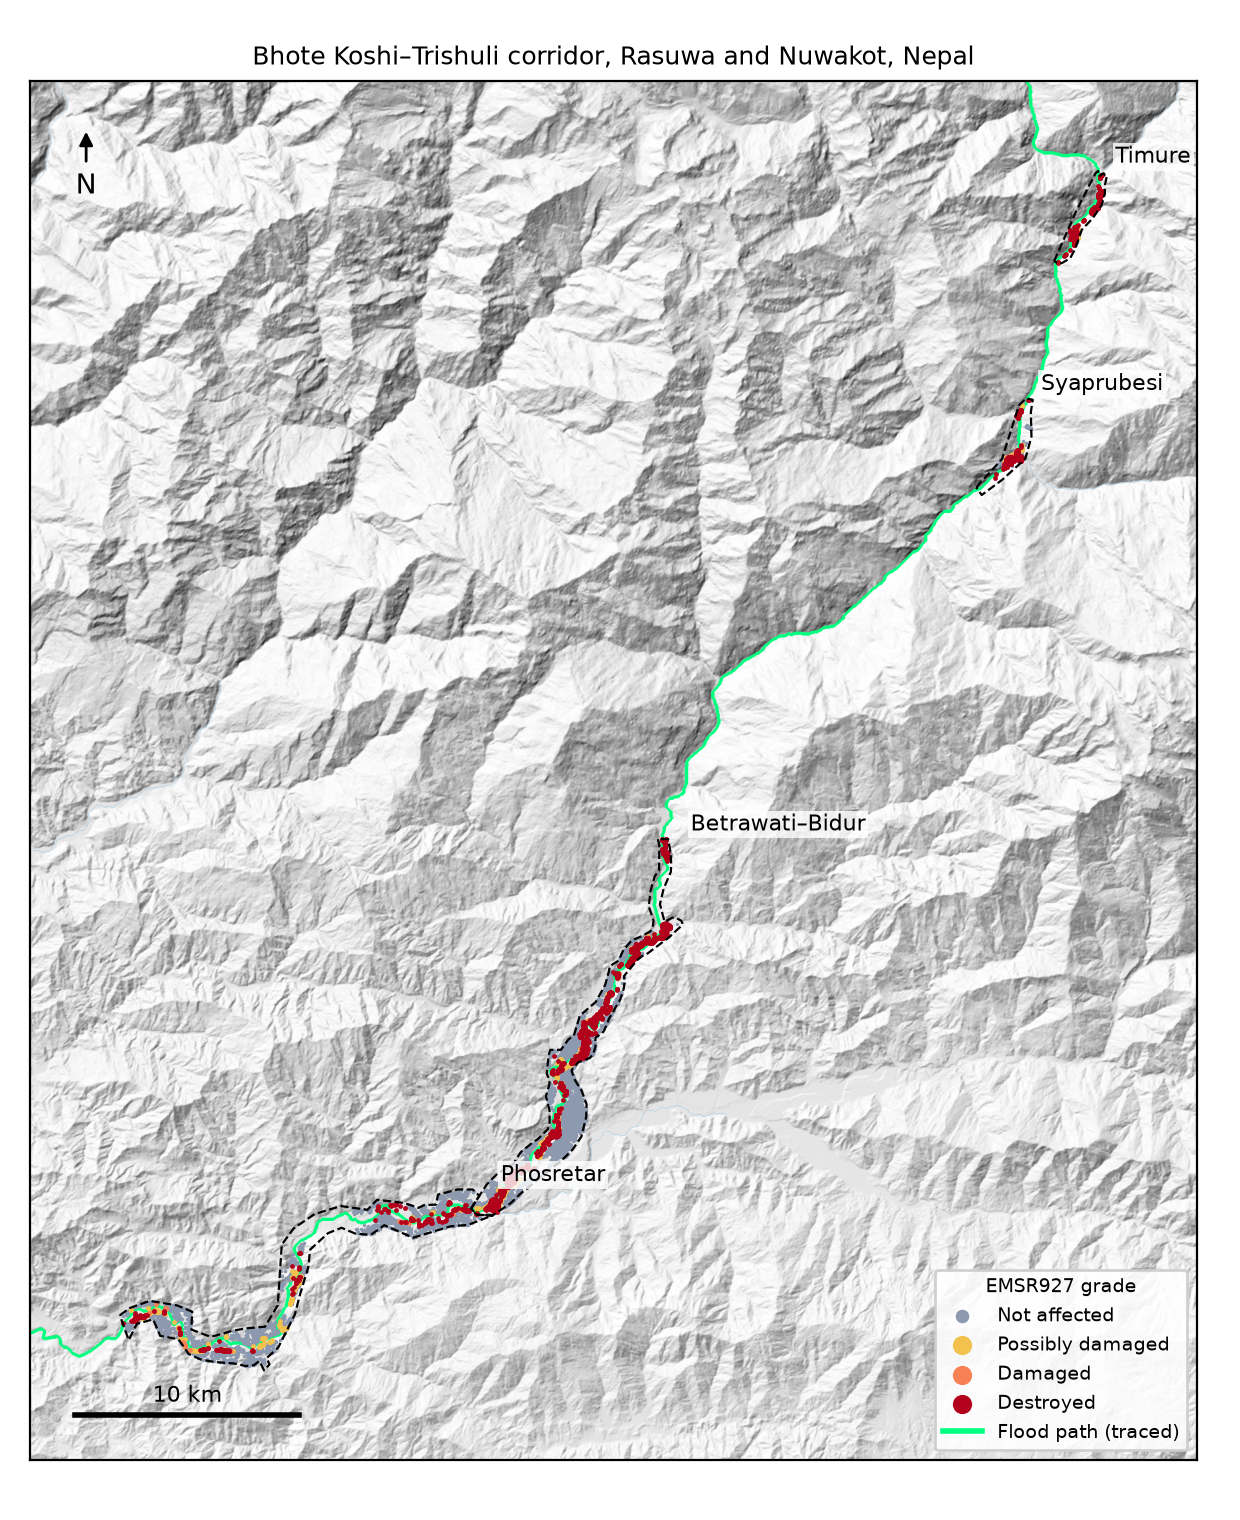
\includegraphics[width=\columnwidth]{figures/study_area.png}
  \caption{Study area. Dashed outlines are the four Copernicus EMSR927 mapping areas. Points are pre-event buildings coloured by damage grade; the green line is the traced flood path.}
  \label{fig:map}
\end{figure}

\begin{table}[t]
\centering\footnotesize
\setlength{\tabcolsep}{3pt}
\caption{The three reaches used for transfer tests. Distance is along the flood path from the border.}\label{tab:reaches}
\begin{tabular}{@{}lrrrrr@{}}
\toprule
\textbf{Reach} & \textbf{km} & \textbf{Bldgs} & \textbf{Affected} & \textbf{Destr.} & \textbf{Blocks}\\
\midrule
Upper\textsuperscript{a} & 0--16 & 845 & 653 (77\%) & 531 & 12\\
Middle\textsuperscript{b} & 42--65 & 10,456 & 2,141 (20\%) & 1,699 & 38\\
Lower\textsuperscript{c} & 65--91 & 6,202 & 566 (9\%) & 275 & 40\\
\midrule
Total & & 17,503 & 3,360 (19\%) & 2,505 & 90\\
\bottomrule
\end{tabular}\\[1pt]
{\scriptsize \textsuperscript{a}Syaprubesi and Timure; \textsuperscript{b}Betrawati--Bidur; \textsuperscript{c}Phosretar. The middle and lower areas meet at km 65; their boundary is not perpendicular to the flood path, so they overlap by about 0.4\,km. Blocks: 1-km spatial blocks.}
\end{table}

\subsection{Data}
All data are open or openly licensed for research (Table~\ref{tab:data}). The study uses no personal data: buildings are anonymous footprints, damage grades come from satellite interpretation, and no people were surveyed, so no ethical approval was needed.

Pre-event footprints came from the Overture Maps release of 19 August 2026, one week before the event, which merges OpenStreetMap with machine-detected footprints. Footprints from before the event are needed: a destroyed building is often missing from post-event mapping, and it would then be counted as absent rather than as damaged. Each footprint is reduced to its centroid, and every feature is read from the elevation model at that point. Footprint shape, size and material were deliberately left out, so the model sees only where a building stands. This is all that is known, consistently, for buildings in a valley that has not yet been hit.

\begin{table}[t]
\centering\footnotesize
\setlength{\tabcolsep}{3pt}
\caption{Data sources.}\label{tab:data}
\begin{tabularx}{\columnwidth}{@{}L{1.3cm}L{2.3cm}YL{1.55cm}@{}}
\toprule
\textbf{Data} & \textbf{Source} & \textbf{Role} & \textbf{Licence}\\
\midrule
Damage labels & Copernicus EMS EMSR927, AOIs 01--03, 05 \citep{ems2026} & 3,816 points graded destroyed / damaged / possibly damaged by photo-interpretation & Copernicus EMS terms (free and open)\\
Footprints & Overture Maps 2026-08-19 \citep{overture2026} & Pre-event buildings; used only to place labels and define undamaged buildings & ODbL 1.0\\
Elevation & Copernicus GLO-30 \citep{copdem}; FABDEM \citep{hawker2022} & Source of all features; FABDEM as robustness check & Copernicus DEM licence (free); CC BY-NC-SA 4.0\\
Imagery & Vantor Open Data (OpenAerialMap), 2021--2026 & Visual label audit only & CC BY-NC 4.0\\
Land cover & ICIMOD/FRTC NLCMS 2022 \citep{nlcms} & Error analysis only & CC BY 4.0\\
\bottomrule
\end{tabularx}
\end{table}

\paragraph{Labels} The Copernicus grading products list affected buildings only. Each graded point was matched to the footprint containing it, or to one within 10\,m, keeping the worst grade per footprint; 3,400 of 3,816 points (89\%) matched. The 416 unmatched points, mostly buildings absent from the pre-event footprints, are kept as point-only rows; they add affected buildings with no footprint-derived attributes, which is one reason footprint size is not a feature. Footprints with no graded point are labelled \emph{not affected}. Table~\ref{tab:grades} maps the grades to the three targets. This is supported by the Copernicus summary tables, which also count buildings with ``no visible damage'': in Syaprubesi and Betrawati--Bidur the totals agree with our footprint counts to within 1\% and 6\%.

\begin{table}[t]
\centering\footnotesize
\setlength{\tabcolsep}{3pt}
\caption{Copernicus damage grades and the three binary targets (counts after cleaning).}\label{tab:grades}
\begin{tabular}{@{}lrccc@{}}
\toprule
\textbf{EMS grade} & \textbf{n} & \textbf{Affected} & \textbf{Destroyed} & \textbf{Destr.\,$\mid$\,aff.}\\
\midrule
Destroyed & 2,505 & 1 & 1 & 1\\
Damaged & 282 & 1 & 0 & 0\\
Possibly damaged & 573 & 1 & 0 & 0\\
No graded point & 14,143 & 0 & 0 & --\\
\bottomrule
\end{tabular}
\end{table}

\paragraph{Cleaning} Three rules were applied (18,908 $\rightarrow$ 17,503 rows; Table~\ref{tab:clean}). R1 removes 1,282 ungraded footprints inside the mapped flood trace (the Copernicus observed-event polygon), whose status is ambiguous; R2 removes 106 ungraded footprints smaller than 10\,m$^2$ (sheds); R3 removes 17 ungraded footprints whose nearest neighbour, within 8\,m, is an affected footprint from another source (duplicates of the same house). No affected building is removed. Post-event information (the flood trace) is used only for cleaning, never as a feature.

\begin{table}[t]
\centering\footnotesize
\setlength{\tabcolsep}{3pt}
\caption{Cleaning log. Rules R1--R3 remove ungraded footprints only.}\label{tab:clean}
\begin{tabular}{@{}lrr@{}}
\toprule
\textbf{Step} & \textbf{Rows} & \textbf{Removed}\\
\midrule
EMS points joined to pre-event footprints & 18,908 & --\\
R1: ungraded footprints inside the flood trace & 17,626 & 1,282\\
R2: ungraded footprints $<$ 10\,m$^2$ & 17,520 & 106\\
R3: ungraded twins $<$ 8\,m from an affected footprint & 17,503 & 17\\
\bottomrule
\end{tabular}
\end{table}

\paragraph{Label audit} A stratified sample of 200 buildings (50 per area; 80 destroyed, 40 damaged or possibly damaged, 80 not affected) was checked against pre- and post-event Vantor imagery at 0.2\,m/pixel in 160\,m and 80\,m windows. Forty-one chips could not be judged. Of these, 18 were ``not affected'' (15 footprints on trees or open ground with no building visible on either date, 3 obscured by cloud, haze or an image artefact), 10 were ``destroyed'' (8 obscured or without a post-event image, 2 under sediment with an ambiguous standing structure) and 13 were ``damaged'' or ``possibly damaged'' (8 with no visible building, 3 with an ambiguous structure, 2 obscured). All 62 judgeable ``not affected'' buildings appeared intact. ``Destroyed'' agreed in 52 of 52 judgeable cases in the upper and middle reaches, almost always as a footprint under a uniform sediment or boulder field. In Phosretar, 8 of 18 judgeable ``destroyed'' buildings still stood with their roofs largely intact, often in a row of standing houses surrounded by sediment, so the \emph{destroyed} target is least certain in the lower reach. Of 27 judgeable ``damaged'' or ``possibly damaged'' buildings, 7 showed visible damage and 20 looked intact from above; the latter are recorded as consistent but weak, because a roof-level view cannot show ground-floor inundation. The judgements are in the repository with the chips.

\paragraph{Elevation model} GLO-30 is a surface model and includes canopy. FABDEM, which removes forests and buildings, gives HAND about 1.5\,m lower on average, but model AUCs change by less than 0.002 (Section~\ref{sec:sens}). GLO-30 is therefore kept as the main DEM. The terrain of the valley sides changes little over a decade, so the age of the radar acquisitions behind GLO-30 is less important than its resolution.

\section{Methods}\label{sec:methods}

\subsection{Terrain features}
The GLO-30 tiles were mosaicked and reprojected to UTM zone 45N at 30\,m. Pits and depressions were filled and flats resolved before D8 flow directions were computed with pysheds. The flood path was traced downstream along D8 flow directions from the border, so tributaries the flood did not follow are excluded. HAND, distance and along-river distance are measured to this path. Ten features form the \emph{main} set (Table~\ref{tab:features}). Stream-power index was dropped because it correlates with channel slope at $\rho = 0.99$. An \emph{attenuation} set replaces the valley-geometry group with $\log(d + 10\,\mathrm{km})$, where $d$ is distance along the river, and its product with HAND.

HAND is the elevation of a cell minus that of the flood-path cell it drains to along D8 directions; distance is the straight-line distance to the nearest path cell. Relief is the elevation range in a 510\,m window. Profile and plan curvature follow \citet{zevenbergen1987} on a Gaussian-smoothed DEM; both are positive on convex ground (spurs, fan surfaces, diverging flow) and negative on concave ground (hollows, converging flow), and plan curvature is set to zero on slopes below 2$^\circ$, where it is undefined. The wetness index is $\ln\!\big((a + 30)/(\tan\beta + 0.001)\big)$ with $a$ the D8 specific catchment area in metres; the small offsets avoid division by zero on flat cells. All derivatives are computed on the conditioned DEM. Valley width is the width of ground with HAND $\leq$ 20\,m, averaged over 500\,m of path, and channel slope is the gradient of the path over $\pm$500\,m. Bend exposure is the curvature of the smoothed path, signed positive when the building is on the outer bank. Each feature is read at the building centroid and joined to the label table; no feature uses post-event information.

\begin{table}[t]
\centering\footnotesize
\setlength{\tabcolsep}{3pt}
\caption{Terrain features. All come from the elevation model.}\label{tab:features}
\begin{tabularx}{\columnwidth}{@{}L{1.4cm}L{2.7cm}Y@{}}
\toprule
\textbf{Group} & \textbf{Features} & \textbf{Physical rationale}\\
\midrule
Core & HAND; distance to flood path & Vertical and horizontal exposure\\
Local & Slope; relief; profile and plan curvature; topographic wetness index & Terraces and fans vs.\ hillsides; convex fans and spurs vs.\ hollows that concentrate flow\\
Geometry & Valley width (HAND $\leq$ 20\,m, log); channel slope; signed bend exposure & Confined gorges give deeper, faster flow; outer banks erode\\
Attenu\-ation\textsuperscript{a} & $\log(d+10)$; HAND\,$\times\log(d+10)$ & The flood weakens downstream\\
\bottomrule
\end{tabularx}

{\scriptsize \textsuperscript{a}Replaces the geometry group in the attenuation set.}
\end{table}

\subsection{Targets and learners}
There are three binary targets: (a) affected vs.\ not affected (primary); (b) destroyed vs.\ not destroyed; (c) destroyed vs.\ damaged or possibly damaged, among affected buildings only. Nine learners from the course syllabus were compared: decision tree, $k$-nearest neighbours, logistic regression with elastic-net penalty, linear discriminant analysis with shrinkage, Gaussian naive Bayes, linear SVM, RBF SVM (Nystr\"om approximation), random forest and histogram gradient boosting. Classical learners suit this problem: the data are tabular with few features, and tree ensembles and linear models remain competitive with deep learning on such data \citep{grinsztajn2022}. Linear regression is used for the attenuation curve, and K-means and Ward hierarchical clustering for damage regimes among affected buildings. PCA and feature selection (mutual information, recursive feature elimination) were used in exploration. Reinforcement learning, the remaining module of the syllabus, is not used: the task is a one-shot prediction from fixed features, with no agent, action or sequence of decisions to learn. All learners except the decision tree, random forest and gradient boosting are fitted on standardised features, and every learner that supports it uses class weights. Table~\ref{tab:grids} lists the tuning grids.

\begin{table}[t]
\centering\footnotesize
\setlength{\tabcolsep}{3pt}
\caption{Learners and tuning grids (inner 3-fold CV on ROC-AUC).}\label{tab:grids}
\begin{tabularx}{\columnwidth}{@{}L{2.2cm}Y@{}}
\toprule
\textbf{Learner} & \textbf{Grid}\\
\midrule
Logistic regression & $C \in \{0.001, 0.01, 0.1, 1, 10\}$; L1 ratio $\in \{0, 0.5, 1\}$\\
LDA & shrinkage none or Ledoit--Wolf\\
Decision tree & depth $\in \{2,3,4,6,8\}$; min.\ leaf $\in \{10,50,200\}$\\
$k$-NN & $k \in \{5,15,25,51,101\}$; uniform or distance weights\\
Naive Bayes & variance smoothing $\in \{10^{-9},10^{-6},10^{-3}\}$\\
Linear SVM & $C \in \{0.01,0.1,1\}$\\
RBF SVM & 500 Nystr\"om components; $\gamma \in \{0.05,0.2,1\}$; $C \in \{0.1,1\}$\\
Random forest & 300 trees; depth $\in \{\text{none},8,16\}$; min.\ leaf $\in \{5,20\}$; features $\in \{\sqrt{p}, 0.5\}$\\
Gradient boosting & learning rate $\in \{0.05,0.1\}$; leaves $\in \{15,31\}$; L2 $\in \{0,1\}$\\
\bottomrule
\end{tabularx}
\end{table}

\subsection{Class imbalance}
Prevalence differs strongly by reach (Table~\ref{tab:reaches}). Four strategies were compared with a 0.5 threshold: no correction, class weights, SMOTE \citep{elreedy2023} and ISMOTE \citep{song2024}, plus a threshold tuned by Youden's $J$ on out-of-fold training predictions. ISMOTE repeatedly oversamples the minority points the current model misclassifies. No code is published, so it was re-implemented from the paper (K = 5, 20 iterations). Oversampling is fitted on the training reaches only.

\subsection{Validation}
\paragraph{Why not random splits} Neighbouring buildings share terrain and were hit by the same part of the flood, so a random train--test split puts near-copies of each test building in the training set and overstates skill \citep{currie2026,meyer2022}. Held-out buildings lie a median 6--23\,km from the nearest training building, and the reaches differ in valley form and flood strength, so a held-out reach is a fair stand-in for a new valley section.
\paragraph{Main test} Leave-one-reach-out: train on two reaches, test on the third. Hyperparameters are tuned in an inner 3-fold cross-validation within the training reaches, grouped by 1-km spatial blocks (grid search on ROC-AUC, with the same grid for every split), so the held-out reach is never used for any choice. The decision threshold is set by Youden's $J$ on out-of-fold training predictions. Three quantities could each be called a threshold, so they are named separately throughout: the \emph{damaging height} HAND$_{50}$ is the height above the flood path at which half the buildings were affected (Section~\ref{sec:atten}); the \emph{decision threshold} is the probability above which a building is flagged; and the \emph{probability level} (calibration-in-the-large, Section~\ref{sec:methods}) is how high the predicted probabilities sit as a whole. The secondary analyses (interpretation, label sensitivity, affected share) use one fixed logistic regression ($C = 1$, class weights), so that differences between their variants come from the data, not from re-tuning. The final evaluation with uncertainty uses fixed hyperparameters for each learner (the modal choice of the grid searches for the tree ensembles; $C = 1$ with an L2 penalty for logistic regression and $C = 0.1$ for the linear SVM, which the flat optimum of the linear models justifies, Section~\ref{sec:models}), so that the intervals describe the models that are interpreted later. Held-out AUCs have 95\% intervals from a block bootstrap (1-km blocks of the held-out reach, 1,000 resamples); logistic regression is compared with each other model on the same bootstrap samples.
\paragraph{Inner folds} Two designs were compared: 1-km spatial blocks, and kNNDM \citep{linnenbrink2024,mila2022}, which chooses folds whose distances to the training data match the distances from the held-out reach to the training reaches. The \emph{optimism gap} is the inner-CV AUC minus the held-out AUC. For the tuned learners the inner AUC is the best score of the grid, so part of the gap is the optimism of selection, which grows with the size of the grid.
\paragraph{Near-channel test} Most buildings in the valley stand far above any flood, and a model that merely separates valley floor from hillside scores well on them. To measure what terrain adds beyond that, every model is also scored on the 3,597 buildings with HAND $\leq$ 30\,m and distance $\leq$ 300\,m from the flood path (21\% of the table; 85\% of them affected in the middle reach, 40\% in the lower). The models are trained on all buildings of the two training reaches and only \emph{scored} on this subset, with the same block-bootstrap intervals as the main test. The upper reach cannot be scored: all 205 of its near-channel buildings were affected, so 3,392 buildings are scored (2,308 middle, 1,084 lower). In the feature-group comparison (Section~\ref{sec:groups}) the models are instead trained within the subset, which asks a slightly different question (which features help among exposed buildings) and gives higher scores.
\paragraph{Area of applicability} Following \citet{meyer2022}, a dissimilarity index (DI) measures each held-out building's distance to the nearest training building in the standardised feature space, weighted by permutation importance. Buildings whose DI exceeds the upper whisker of the cross-validated training DI lie outside the area of applicability (AOA).
\paragraph{Metrics} The prevalence of the affected class ranges from 9\% to 77\% between reaches, so accuracy would mostly reflect prevalence. ROC-AUC is the main metric because it measures ranking and does not depend on prevalence, which makes reaches comparable. PR-AUC is reported beside it because it does depend on prevalence and shows how useful a ranking is when damage is rare, as in the lower reach. Balanced accuracy, precision and recall at the tuned threshold describe the map a user would receive.
\paragraph{Circularity} The flood trace and the terrain are not independent: the debris flood followed the valley floor, and the photo-interpreters graded the buildings inside the trace they saw. A terrain model therefore predicts flood extent as well as damage given exposure. Three checks limit this: the trace is never a feature, the near-channel test removes the obvious hillside negatives, and the destroyed $\mid$ affected target asks only about severity among buildings the flood reached.
\paragraph{Calibration} Besides ROC-AUC, PR-AUC and balanced accuracy, we report the Brier score, the calibration intercept (calibration-in-the-large; 0 is ideal), the calibration slope (1 is ideal) and the expected calibration error (ECE). Imbalance corrections are known to distort probabilities \citep{vandengoorbergh2022,carriero2025}. To test cheap recalibration, the intercept alone is re-fitted on $k$ randomly chosen buildings of the held-out reach ($k$ = 10--200, 200 repeats) and the rest are scored.

\subsection{Attenuation curve}
Buildings were binned in 3-km steps of along-river distance. In each bin with at least 15 buildings of each class, a one-feature logistic regression on HAND gives HAND$_{50}$, the height at which the damage probability is 50\%. HAND$_{50}$ was regressed on distance with ordinary least squares, linearly and in $\log(d + c)$, with $c$ chosen by leave-one-bin-out cross-validation from $\{1, 2, 5, 10, 20, 40\}$\,km. Since $d$ is measured from the border and the avalanche started some 15--20\,km further up the valley, $d + c$ approximates the distance from the source, and the slope in $\log(d+c)$ is reported as the change per doubling of that distance. Slope intervals come from 300 bootstrap resamples with the form and $c$ held fixed and the bins, HAND$_{50}$ values and regression refitted in each resample. The headline interval resamples the 1-km spatial blocks, because neighbouring buildings share terrain and flood exposure and are not independent draws; resampling buildings within bins and resampling the bins themselves are reported as comparisons.

\subsection{Interpretation}
Permutation importance and partial dependence are used with care, since HAND and distance are correlated (Spearman $\rho = 0.67$) and both methods can mislead under correlation \citep{molnar2022}. Four views are combined. (i) Standardised logistic-regression coefficients, fitted on all buildings, with 95\% intervals from 300 bootstrap resamples of 1-km blocks. (ii) Permutation importance computed on the \emph{held-out} reach of each leave-one-reach-out split, as the mean drop in ROC-AUC over 10 shuffles. (iii) Partial dependence of logistic regression and random forest on all buildings. (iv) A depth-3 decision tree (at least 100 buildings per leaf) as readable rules. Errors of the held-out logistic-regression predictions at the tuned threshold are mapped as true and false positives and negatives. To test whether canopy in the surface model causes errors, the share of forest within about 75\,m of each building (ICIMOD NLCMS 2022, 30\,m pixels) is compared between correct and wrong predictions with a Mantel--Haenszel test within strata of reach, HAND (seven bands) and distance (five bands), so that location does not masquerade as land cover.

\subsection{Implementation}
Python 3.12.16 with scikit-learn 1.9.1 \citep{pedregosa2011}, imbalanced-learn 0.14.2 \citep{lemaitre2017}, pysheds 0.5 \citep{pysheds}, geopandas 1.1.4, rasterio 1.5.1 and DuckDB 1.5.5; the pinned environment is in \texttt{requirements.txt}. Random seeds are fixed throughout. The full nested evaluation of nine learners, three targets, two feature sets and three held-out reaches takes about 20 minutes on a laptop. kNNDM and the AOA were re-implemented in Python following the published methods. The pipeline (\texttt{pilot/01}--\texttt{30}) rebuilds every quantitative result and figure from the raw downloads with one script; the visual-audit chips are rebuilt with a separate flag because they need internet access, and the recorded judgements are preserved.

\section{Results}\label{sec:results}

\subsection{Exploratory analysis}\label{sec:eda}
Affected and unaffected buildings differ most in height and distance. Across reaches the median HAND of destroyed buildings is 14--35\,m, of damaged buildings 18--52\,m and of unaffected buildings 53--90\,m; the medians rise upstream for every grade, which anticipates the attenuation curve. Fig.~\ref{fig:hand} shows the same pattern for destruction: the share of buildings destroyed falls from near one to near zero across a band of HAND that sits at 10--20\,m in the lower reach, 15--30\,m in the middle reach and 40--60\,m in the upper gorge. On their own, HAND and distance rank affected buildings with AUC 0.933 and 0.914 (all data, direction-free). Channel slope (0.654), profile curvature (0.657), slope (0.651) and relief (0.627) carry weaker signals, and plan curvature, the wetness index and valley width are close to 0.5 when used alone. Near the channel the picture changes: HAND and distance fall to 0.76, while channel slope (0.708), relief (0.698) and valley width (0.644) gain. These single-feature values pool all three reaches, so they mix the downstream weakening into every feature; scored reach by reach, HAND alone still ranks near-channel buildings at 0.77--0.88 (Section~\ref{sec:near}), and the pooled gain of the secondary features does not carry over to a held-out reach.

Five pairs are strongly correlated (Spearman $|\rho| \geq 0.6$): HAND and distance (0.67), stream power and channel slope (0.99, hence stream power was dropped), along-river distance with channel slope ($-0.76$) and stream power ($-0.70$), and slope with the wetness index ($-0.69$). PCA needs four components to explain 67\% of the variance; the first (25\%) contrasts steep, high-relief gorge settings with the flatter downstream valley, and HAND loads mainly on the third. All three feature-selection methods rank HAND first or second. Distance is first under recursive elimination and third in the L1 path, but only seventh by mutual information, which scores each feature alone and so cannot see that distance adds to HAND. Below that the methods disagree, as expected for correlated features. Because no small subset was clearly better, the main set keeps all ten physically motivated features and leaves the weighting to regularisation.

\begin{figure}[t]
  \centering
  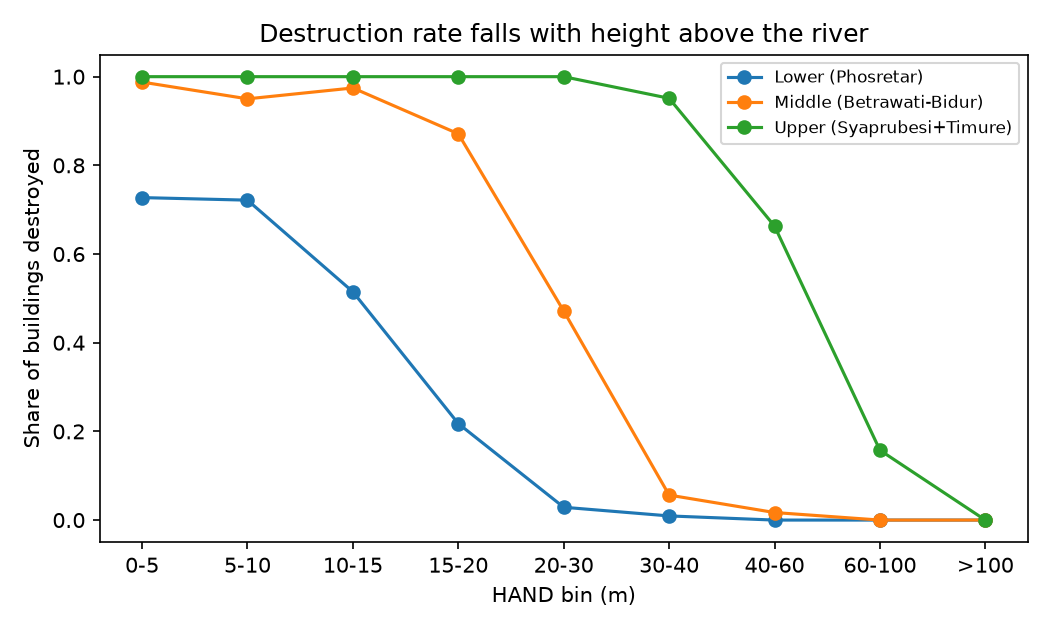
\includegraphics[width=\columnwidth]{figures/fig_destroyed_rate_by_hand.png}
  \caption{Share of buildings destroyed by HAND band in each reach. The band in which destruction drops off moves upward with distance from the source, which anticipates the attenuation curve of Section~\ref{sec:atten}.}
  \label{fig:hand}
\end{figure}

\subsection{Transfer to an unseen reach (RQ1)}
Terrain alone separates affected from unaffected buildings in every held-out reach (Table~\ref{tab:final}). Class-weighted logistic regression reaches AUC 0.970, 0.983 and 0.958 for affected and 0.952, 0.983 and 0.958 for destroyed. The upper reach has the widest intervals: it has only 12 blocks and 192 undamaged buildings. Separating destroyed from damaged among affected buildings is harder (0.930, 0.818 and 0.750).

PR-AUC shows the effect of prevalence. For affected it is 0.991 in the upper reach, 0.929 in the middle and 0.639 in the lower, against prevalences of 0.77, 0.21 and 0.09; for destroyed it falls to 0.406 in the lower reach, where only 4\% of buildings were destroyed. The same ranking quality is therefore worth less where damage is rare. At the tuned threshold, balanced accuracy for affected is 0.89, 0.94 and 0.88. In the middle reach the map is both complete and precise (recall 0.93, precision 0.79). In the lower reach it finds almost every affected building (recall 0.98) but only 30\% of the buildings it flags were affected, and in the upper reach it misses 14\% of the affected buildings while 97\% of its flags are correct. These two opposite errors are examined in Section~\ref{sec:share}.

\begin{table}[t]
\centering\footnotesize
\setlength{\tabcolsep}{3pt}
\caption{Held-out ROC-AUC (main feature set; attenuation set for destroyed $\mid$ affected). 95\% block-bootstrap intervals are shown for logistic regression; the intervals of the other models are in the repository (\texttt{final\_auc\_ci.csv}).}\label{tab:final}
\begin{tabular}{@{}llccc@{}}
\toprule
\textbf{Target} & \textbf{Model} & \textbf{Upper} & \textbf{Middle} & \textbf{Lower}\\
\midrule
\multirow{4}{*}{Affected} & LogReg & \textbf{0.970} & \textbf{0.983} & \textbf{0.958}\\
 & & {\scriptsize(0.90--1.00)} & {\scriptsize(0.97--0.99)} & {\scriptsize(0.94--0.97)}\\
 & Random forest & 0.858 & 0.957 & 0.947\\
 & Grad.\ boosting & 0.879 & 0.966 & 0.944\\
\midrule
\multirow{3}{*}{Destroyed} & LogReg & 0.952 & 0.983 & 0.958\\
 & & {\scriptsize(0.88--0.99)} & {\scriptsize(0.97--0.99)} & {\scriptsize(0.93--0.98)}\\
 & Random forest & 0.904 & 0.960 & 0.951\\
\midrule
\multirow{2}{*}{Destr.\,$\mid$\,aff.} & LogReg & 0.930 & 0.818 & 0.750\\
 & & {\scriptsize(0.87--0.98)} & {\scriptsize(0.78--0.85)} & {\scriptsize(0.68--0.82)}\\
\bottomrule
\end{tabular}
\end{table}

\subsection{Near the channel: what terrain adds beyond the valley floor}\label{sec:near}
The scores in Table~\ref{tab:final} are inflated by buildings that stand 50\,m or more above the river and were never at risk. Table~\ref{tab:near} removes them. Among the buildings within 30\,m height and 300\,m distance of the flood path, the same logistic regression ranks affected buildings in an unseen reach with AUC 0.851 (95\% interval 0.765--0.920) in the middle reach and 0.801 (0.689--0.889) in the lower reach, and destroyed buildings with 0.859 and 0.781. With the penalty chosen over the tuning grid rather than fixed at $C = 1$, the affected scores are 0.851 and 0.784 (mean 0.818, the near-channel column of Table~\ref{tab:models}). This is the size of the terrain signal once ``was the building on the valley floor'' is taken away: clearly better than chance, but with about a fifth of the ranking error left, and with intervals five to seven times wider than over all buildings, because the subset holds only 1,084--2,308 buildings. PR-AUC follows prevalence as before: 0.968 in the middle reach, where 85\% of near-channel buildings were affected, and 0.670 in the lower reach, where 40\% were.

The models are closer together here than over all buildings. Random forest is marginally ahead of logistic regression for affected in the middle reach ($-0.009$, interval $-0.051$ to $+0.022$), the only near-channel cell in which random forest is nominally ahead of logistic regression, and logistic regression is ahead of gradient boosting there (+0.056, +0.008 to +0.107); every other paired difference includes zero. The large gap between linear and tree models that appears in Table~\ref{tab:final} therefore comes mainly from the hillside buildings of the upper gorge, which lie outside the trees' training range (Section~\ref{sec:aoa}), and not from how the models rank buildings that the flood could reach.

Two baselines that involve no learning give a scale for these scores. Ranking the near-channel buildings by HAND alone gives AUC 0.876 and 0.770 for affected and 0.854 and 0.827 for destroyed: as good as the ten-feature logistic regression in every cell (paired differences $-0.045$ to $+0.031$, all intervals including zero) and nominally better in two of four. Near the channel, the eight other terrain features add no held-out ranking skill once HAND is known. A single HAND threshold, by contrast, is much weaker: the Youden cut chosen on the training reaches (15--23\,m) reaches a balanced accuracy of only 0.64--0.68, and logistic regression beats it by 0.10--0.21 (three of four intervals exclude zero). A cut chosen on all training buildings is 31--55\,m, above the subset ceiling, and flags every near-channel building. The model does not order the exposed buildings better than HAND does. What it adds over a rule is a probability and a decision threshold fitted to the training reaches. The feature-group comparison of Section~\ref{sec:groups}, which trains within the subset, shows a gain from local terrain (0.832 $\rightarrow$ 0.862); that gain does not survive when the model is trained on all buildings and only scored near the channel, so it should be read as the weaker evidence.

\begin{table}[t]
\centering\footnotesize
\setlength{\tabcolsep}{3pt}
\caption{Near-channel test: held-out ROC-AUC for buildings with HAND $\leq$ 30\,m and distance $\leq$ 300\,m (95\% block-bootstrap intervals shown for logistic regression and the HAND-only baseline; all intervals are in \texttt{nearchannel\_ci.csv}), main feature set, final fixed models trained on all buildings of the other two reaches, against two training-free baselines. \emph{HAND only} ranks buildings by HAND with no model. \emph{HAND cut} is one threshold chosen by Youden's $J$ on the near-channel buildings of the training reaches (15--23\,m); a binary rule is one point on the ROC curve, so its AUC equals its balanced accuracy. The upper reach has no unaffected near-channel buildings and cannot be scored. $n$ = 2,308 (middle), 1,084 (lower).}\label{tab:near}
\begin{tabular}{@{}llcc@{}}
\toprule
\textbf{Target} & \textbf{Model} & \textbf{Middle} & \textbf{Lower}\\
\midrule
\multirow{8}{*}{Affected} & LogReg & 0.851 & \textbf{0.801}\\
 & & {\scriptsize(0.77--0.92)} & {\scriptsize(0.69--0.89)}\\
 & Linear SVM & 0.850 & 0.792\\
 & Random forest & 0.860 & 0.756\\
 & Grad.\ boosting & 0.794 & 0.742\\
 & HAND only (no model) & \textbf{0.876} & 0.770\\
 & & {\scriptsize(0.84--0.91)} & {\scriptsize(0.67--0.84)}\\
 & HAND cut (16 / 23\,m) & 0.652 & 0.644\\
 & PR-AUC (LogReg) / prevalence & 0.968 / 0.85 & 0.670 / 0.40\\
\midrule
\multirow{6}{*}{Destroyed} & LogReg & \textbf{0.859} & 0.781\\
 & & {\scriptsize(0.81--0.91)} & {\scriptsize(0.66--0.90)}\\
 & Random forest & 0.854 & 0.755\\
 & Grad.\ boosting & 0.821 & 0.786\\
 & HAND only (no model) & 0.854 & \textbf{0.827}\\
 & & {\scriptsize(0.83--0.88)} & {\scriptsize(0.76--0.90)}\\
 & HAND cut (15 / 22\,m) & 0.647 & 0.683\\
\bottomrule
\end{tabular}
\end{table}

\subsection{Which learners transfer (RQ3)}\label{sec:models}
Linear models transfer best (Table~\ref{tab:models}). On the same bootstrap samples, logistic regression beats random forest by +0.112 (95\% interval +0.022 to +0.206) and gradient boosting by +0.091 (+0.019 to +0.183) in the upper reach, and by +0.026 and +0.017 in the middle reach; in the lower reach the differences are not significant. Logistic regression and linear SVM are indistinguishable.

The order of the learners is almost the same for every target. For destroyed, the linear models again lead (mean held-out AUC 0.964), followed by RBF SVM (0.956), gradient boosting (0.943) and random forest (0.940); the decision tree (0.889) and $k$-NN (0.899) are last. For destroyed $\mid$ affected with the main set (the attenuation set adds about 0.04 for logistic regression), all learners are weaker and the spread is larger: logistic regression 0.792, linear SVM 0.781, LDA 0.769, RBF SVM 0.730, random forest 0.724, $k$-NN 0.695, naive Bayes 0.692, gradient boosting 0.651 and the decision tree 0.548. $k$-NN and naive Bayes suffer most near the channel (0.62 and 0.65), where a few correlated features have to be weighed against each other. LDA and naive Bayes, which assume Gaussian classes, trail logistic regression by 0.02--0.04 for affected; the right-skewed HAND and distance distributions (skewness 1.2 and 0.9) violate that assumption. The selected logistic-regression penalty varied widely between splits ($C$ from 0.01 to 10; 11 of 27 fits chose 0.01), yet the fixed $C = 1$ model used in the secondary analyses gives the same mean affected AUC (0.970 vs.\ 0.969), so the result does not hinge on tuning.

\begin{table}[t]
\centering\footnotesize
\setlength{\tabcolsep}{3pt}
\caption{Model comparison on the main feature set, tuned learners. Held-out: mean AUC over reaches (affected). Near-channel: the same models scored on buildings with HAND $\leq$ 30\,m and distance $\leq$ 300\,m. Gap: inner 1-km block CV AUC minus held-out AUC, affected, mean over reaches.}\label{tab:models}
\begin{tabular}{@{}lccc@{}}
\toprule
\textbf{Model} & \textbf{Held-out} & \textbf{Near-channel} & \textbf{Gap}\\
\midrule
Logistic regression & \textbf{0.969} & \textbf{0.818} & 0.006\\
Linear SVM & \textbf{0.969} & \textbf{0.818} & 0.005\\
RBF SVM & 0.954 & 0.788 & 0.018\\
LDA & 0.945 & 0.759 & \textbf{0.003}\\
Naive Bayes & 0.934 & 0.652 & 0.011\\
Random forest & 0.920 & 0.808 & 0.055\\
$k$-NN & 0.918 & 0.622 & 0.037\\
Gradient boosting & 0.887 & 0.781 & 0.087\\
Decision tree & 0.878 & 0.750 & 0.069\\
\bottomrule
\end{tabular}
\end{table}

Inside the training reaches, flexible models look as good as linear ones (inner AUC for affected: random forest 0.975, logistic regression 0.974), but on a new reach they lose far more: 0.055 (random forest) and 0.087 (gradient boosting) of AUC against 0.006 for logistic regression. kNNDM folds come closer to the real transfer setting than 1-km blocks: their median fold-to-training distance is 1.2--3.0\,km instead of 250--330\,m, and they reduce the mean absolute optimism gap from 0.034 to 0.025. They still cannot reproduce the 6--23\,km jump to a new reach, and no inner design ranks the models correctly: under kNNDM, random forest (0.965) still beats logistic regression (0.960) inside the training reaches, while the held-out reaches show the reverse (0.929 vs.\ 0.967).

\subsection{Which terrain groups add information}\label{sec:groups}
Table~\ref{tab:groups} adds the feature groups one at a time, with a fixed logistic regression and a fixed random forest (400 trees, minimum leaf 10; not the tuned forest of Table~\ref{tab:final}), so that the gain of each group can be read directly. Adding local terrain to the core features raised the mean affected AUC of logistic regression from 0.954 to 0.964, and adding valley geometry raised it to 0.970; the same two steps raised destroyed from 0.942 to 0.964. The attenuation terms helped the destroyed targets most (destroyed $\mid$ affected 0.788 $\rightarrow$ 0.833) but hurt the near-channel subset (0.856 $\rightarrow$ 0.813; here the models are trained within the subset, so the scores sit above those of Table~\ref{tab:near}), because along-river distance is extrapolated for every held-out reach and, near the channel, mostly separates reaches with different damage shares. All features together gave no consistent gain: for logistic regression the full set was within 0.002 of the best subset on affected and destroyed but lower elsewhere; the random forest gained 0.012 on the near-channel subset (0.826 $\rightarrow$ 0.838). The random forest behaves differently: it gains little from geometry (0.920) and needs the attenuation terms to transfer at all (0.963 for affected), because without them it learns reach-specific HAND thresholds that do not hold in the held-out gorge. Valley geometry therefore carries much of the downstream weakening in a form that transfers without extrapolation. The near-channel gains in this table come from models trained within the subset; when the final model is trained on all buildings, HAND alone ranks the near-channel buildings as well as any feature set (Table~\ref{tab:near}), so the secondary features contribute to the decision threshold and to the all-building ranking; they do not order the exposed buildings better than HAND.

\begin{table*}[t]
\centering\footnotesize
\setlength{\tabcolsep}{5pt}
\caption{Feature groups added in turn: mean held-out ROC-AUC over the three reaches, logistic regression (LR, $C = 1$, class weights) and random forest (RF, 400 trees, min.\ leaf 10). Core: HAND and distance; local: slope, relief, curvatures, wetness index; geometry: valley width, channel slope, bend; attenuation: $\log(d+10)$ and its product with HAND, used in place of geometry. N-ch.: near-channel subset, with the models trained and tested within the subset (middle and lower reaches).}\label{tab:groups}
\begin{tabular}{@{}lcccccccc@{}}
\toprule
 & \multicolumn{2}{c}{\textbf{Affected}} & \multicolumn{2}{c}{\textbf{Destroyed}} & \multicolumn{2}{c}{\textbf{Aff., n-ch.}} & \multicolumn{2}{c}{\textbf{D\,$\mid$\,A}}\\
\cmidrule(lr){2-3}\cmidrule(lr){4-5}\cmidrule(lr){6-7}\cmidrule(lr){8-9}
\textbf{Features} & LR & RF & LR & RF & LR & RF & LR & RF\\
\midrule
Core & 0.954 & 0.924 & 0.942 & 0.909 & 0.832 & 0.774 & 0.748 & 0.630\\
+ local & 0.964 & 0.928 & 0.951 & 0.924 & \textbf{0.862} & 0.814 & 0.759 & 0.750\\
+ geometry (main) & \textbf{0.970} & 0.920 & 0.964 & 0.940 & 0.856 & 0.822 & 0.788 & 0.732\\
+ attenuation & 0.968 & \textbf{0.963} & 0.971 & 0.962 & 0.813 & 0.826 & \textbf{0.833} & \textbf{0.806}\\
All & 0.968 & 0.961 & \textbf{0.972} & \textbf{0.964} & 0.824 & \textbf{0.838} & 0.820 & 0.788\\
\bottomrule
\end{tabular}
\end{table*}

\subsection{Why flexible models fail: area of applicability}\label{sec:aoa}
With the main feature set, 7--21\% of the middle and lower reaches lie outside the AOA, but 74--83\% of the upper gorge does: its steep, narrow terrain is unlike anything downstream (Fig.~\ref{fig:aoa}). The tree models' collapse is concentrated there. Outside the AOA in the upper reach, random forest and gradient boosting reach AUC 0.811 and 0.843, against 0.957 for logistic regression; inside it, random forest reaches 0.959. With the attenuation set, the whole upper reach and 65--67\% of the lower reach fall outside the AOA, because along-river distance is extrapolated.

\begin{figure*}[t]
  \centering
  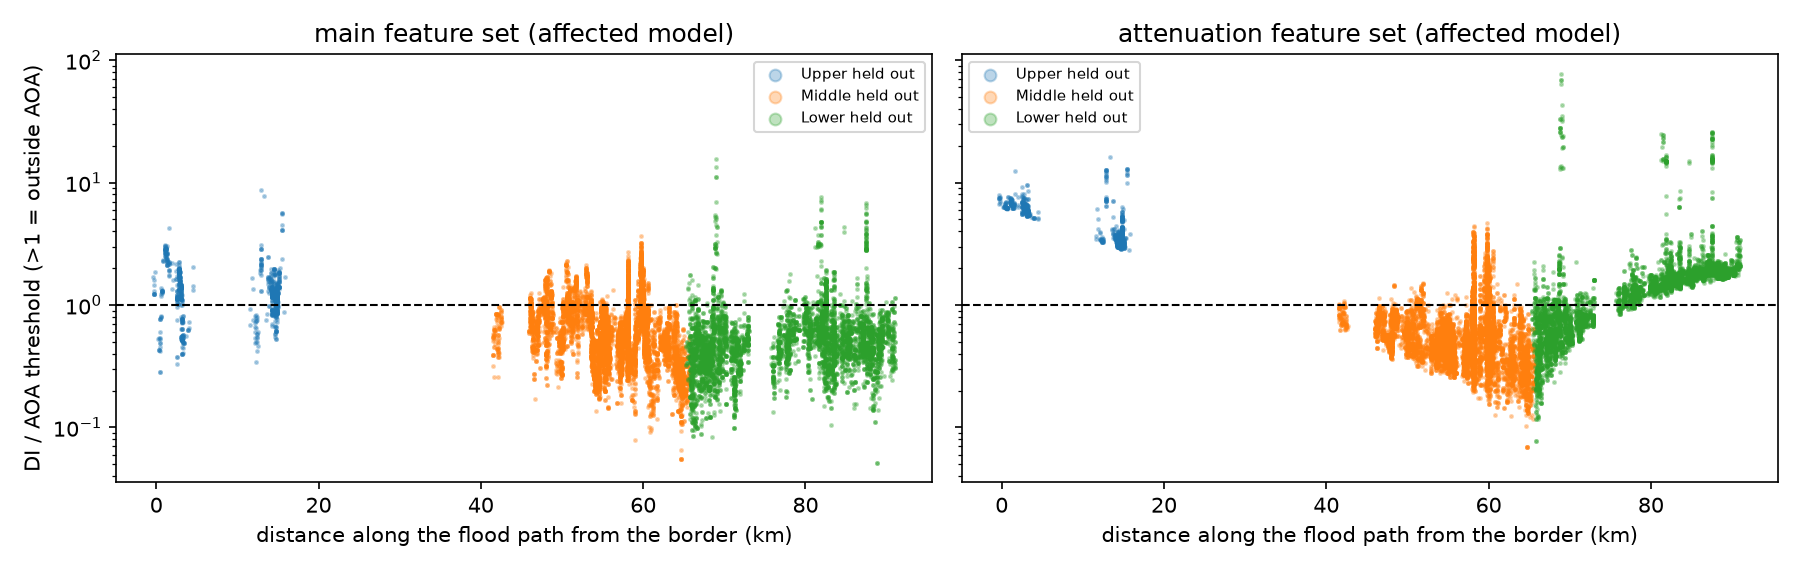
\includegraphics[width=0.92\textwidth]{figures/fig_aoa_di.png}
  \caption{Dissimilarity index of held-out buildings relative to the AOA threshold (values above 1 lie outside the area of applicability), against distance along the flood path. Left: main feature set. Right: attenuation set, where along-river distance is extrapolated for the upper and lower reaches.}
  \label{fig:aoa}
\end{figure*}

\subsection{Attenuation of the flood (RQ2)}\label{sec:atten}
The damaging height above the river falls with distance downstream (Fig.~\ref{fig:atten}). A logarithmic form fits far better than a straight line (leave-one-bin-out RMSE 4.7 vs.\ 10.4\,m for affected, with $c = 5$\,km; 4.0 vs.\ 5.5\,m for destroyed, with $c = 20$\,km). For destroyed the error is flat between $c = 10$ and 40\,km (4.1--4.5\,m); for affected it rises from 4.7\,m at $c = 5$ to 7.3\,m at $c = 40$. HAND$_{50}$ falls by 19.5\,m per doubling of distance for affected buildings (95\% block-bootstrap interval 16.8--21.9\,m; $R^2 = 0.94$) and by 23.0\,m for destroyed buildings (19.9--28.8\,m; $R^2 = 0.93$). The fitted curve falls from about 87\,m (affected) and 63\,m (destroyed) near the border to about 16\,m and 11\,m at 90\,km; the last observed bin, at 91\,km, has HAND$_{50}$ of 19.6\,m and 15.3\,m. The bootstrap unit changes the interval (Table~\ref{tab:attboot}): resampling buildings within bins gives intervals 1.5 (affected) to 2.2 (destroyed) times narrower than resampling 1-km blocks, and resampling the bins themselves gives the widest interval for affected (14.9--21.3\,m). Under every scheme the slope is far from zero. The intervals of the two targets overlap under block and bin resampling; under building-level resampling they just separate (17.7--21.1 vs.\ 21.5--25.5\,m). The block interval is the one we report.

\begin{table}[t]
\centering\footnotesize
\setlength{\tabcolsep}{4pt}
\caption{Attenuation slope in metres of HAND$_{50}$ per doubling of distance from the source (negative = falling), with 95\% intervals from three bootstrap schemes (300 resamples each; form and $c$ fixed).}\label{tab:attboot}
\setlength{\tabcolsep}{3pt}
\begin{tabular}{@{}lcccc@{}}
\toprule
\textbf{Target} & \textbf{Slope} & \textbf{1-km blocks} & \textbf{Buildings} & \textbf{Bins}\\
\midrule
Affected, $c$ = 5 & 19.5 & 16.8--21.9 & 17.7--21.1 & 14.9--21.3\\
Destroyed, $c$ = 20 & 23.0 & 19.9--28.8 & 21.5--25.5 & 20.8--30.2\\
\bottomrule
\end{tabular}\\[1pt]
{\scriptsize $c$ in km. All values are magnitudes of the fall in HAND$_{50}$.}
\end{table}

\begin{figure}[t]
  \centering
  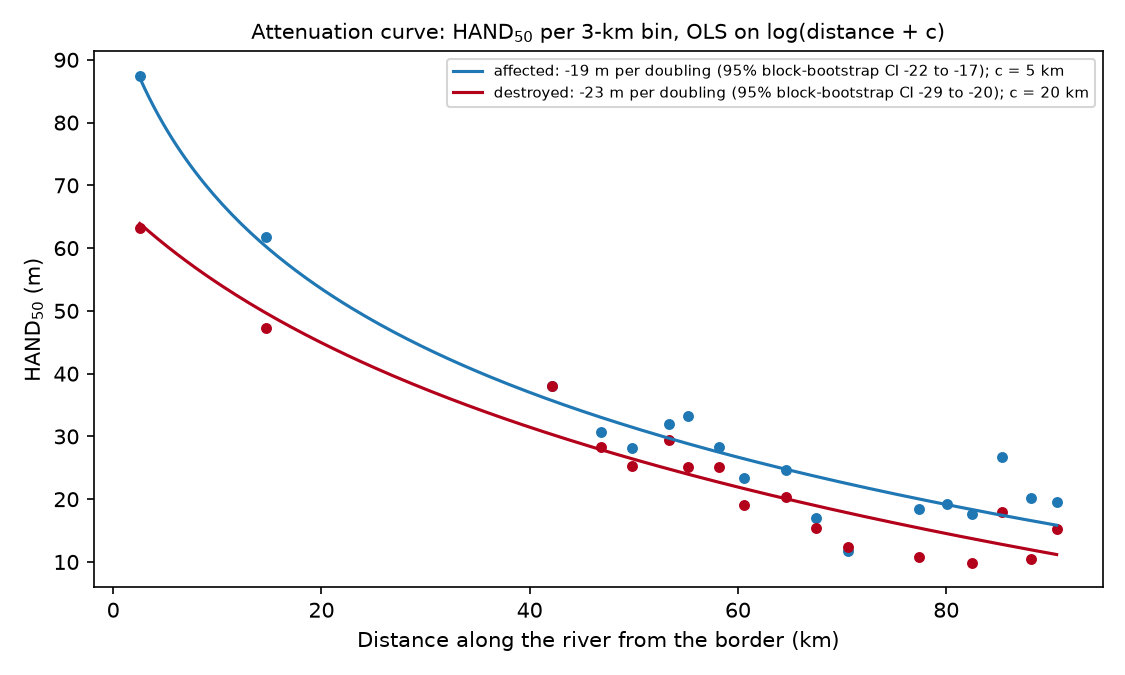
\includegraphics[width=\columnwidth]{figures/fig_attenuation_final.png}
  \caption{Attenuation curve. HAND$_{50}$ per 3-km bin against distance along the flood path, with the fitted logarithmic curve.}
  \label{fig:atten}
\end{figure}

\subsection{Ranking transfers, probabilities do not (RQ4)}
The calibration intercept follows flood strength (Fig.~\ref{fig:cal}, Table~\ref{tab:cal}). Trained on the middle and lower reaches, logistic regression \emph{under}-predicts damage in the upper reach (intercept +2.3 to +4.1, depending on the imbalance strategy); trained on the upper and middle reaches, it \emph{over}-predicts in the lower reach ($-$1.5 to $-$2.6). The middle reach, which lies between the others, is close to calibrated. Class weights and SMOTE raise every probability, which helps upstream and hurts downstream. Tree models are the worst calibrated: random forest probabilities are too timid (slope 1.6) and gradient boosting's too extreme (0.6).

\begin{figure*}[t]
  \centering
  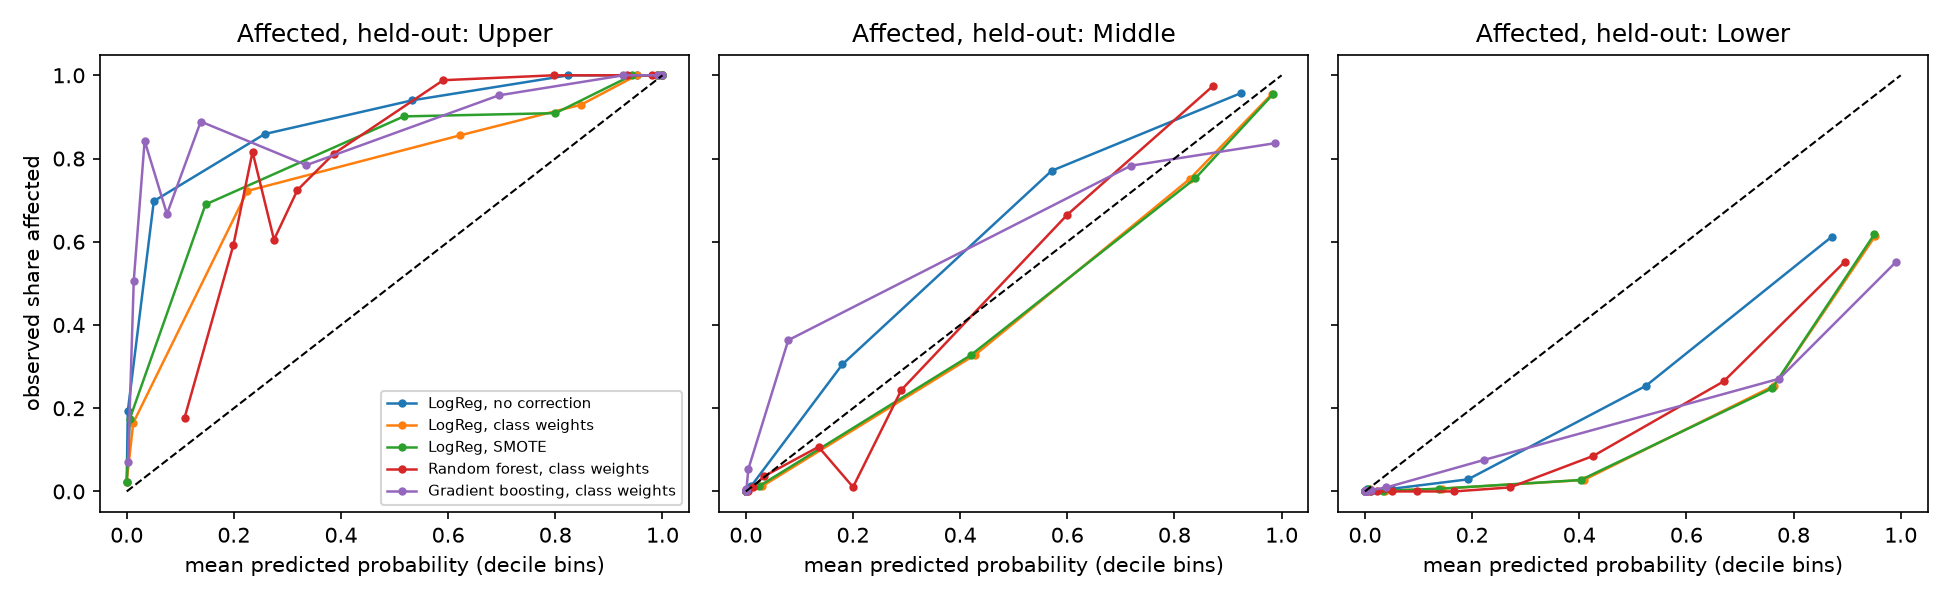
\includegraphics[width=0.92\textwidth]{figures/fig_calibration.png}
  \caption{Reliability diagrams for the affected target in each held-out reach (decile bins). Points above the diagonal are under-predicted; below it, over-predicted.}
  \label{fig:cal}
\end{figure*}

\begin{table}[t]
\centering\footnotesize
\setlength{\tabcolsep}{3pt}
\caption{Calibration, mean over reaches and targets (main set). Intercept: calibration-in-the-large per held-out reach (U / M / L), mean over the two targets; positive means under-prediction.}\label{tab:cal}
\begin{tabular}{@{}lccccc@{}}
\toprule
\textbf{Model} & \textbf{AUC} & \textbf{Brier} & \textbf{Slope} & \textbf{ECE} & \textbf{Intercept U / M / L}\\
\midrule
LogReg, no correction & 0.968 & 0.080 & 0.86 & 0.090 & $+3.1$ / $+0.9$ / $-1.6$\\
LogReg, class weights & 0.967 & \textbf{0.075} & 0.79 & \textbf{0.082} & $+1.3$ / $-0.7$ / $-2.9$\\
LogReg, SMOTE & 0.967 & 0.078 & 0.74 & 0.086 & $+1.9$ / $-0.8$ / $-2.9$\\
Random forest, weights & 0.929 & 0.124 & 1.56 & 0.155 & $+1.6$ / $-0.3$ / $-2.4$\\
Grad.\ boosting, weights & 0.941 & 0.153 & 0.59 & 0.169 & $+4.3$ / $+0.1$ / $-3.8$\\
\bottomrule
\end{tabular}
\end{table}

Re-fitting only the intercept removes most of this error with very few labels (Table~\ref{tab:recal}). With 20 labelled buildings from the held-out reach, the ECE of the uncorrected logistic regression falls from 0.211 to 0.047 in the upper reach and from 0.074 to 0.028 in the lower reach; beyond 50 labels the gain is small.

\begin{table}[t]
\centering\footnotesize
\setlength{\tabcolsep}{4pt}
\caption{Intercept-only recalibration with $k$ labelled buildings of the held-out reach: ECE (median of 200 repeats; affected, logistic regression without correction).}\label{tab:recal}
\begin{tabular}{@{}lcccccc@{}}
\toprule
\textbf{Reach} & \textbf{none} & \textbf{10} & \textbf{20} & \textbf{50} & \textbf{100} & \textbf{200}\\
\midrule
Upper & 0.211 & 0.073 & 0.047 & 0.040 & 0.039 & 0.038\\
Middle & 0.036 & 0.031 & 0.024 & 0.019 & 0.015 & 0.013\\
Lower & 0.074 & 0.040 & 0.028 & 0.025 & 0.022 & 0.022\\
\bottomrule
\end{tabular}
\end{table}

\subsection{Predicted versus observed affected share}\label{sec:share}
For a responder, the first question after an event is often how many buildings in each settlement were hit, and only then which ones. Table~\ref{tab:share} and Fig.~\ref{fig:share} compare the observed share of affected buildings with three predictions from models that never saw the reach. Without recalibration, logistic regression predicts 56\% instead of 77\% in the upper reach and 17\% instead of 9\% in the lower reach: it pulls every reach towards the average flood of its training reaches. Re-fitting the intercept on 50 labelled buildings brings all three reaches within one percentage point, and the error per 3-km bin falls from 6.2 to 2.4 percentage points. The thresholded map is worst: in the lower reach it flags 30\% of all buildings, more than three times the true share, and up to 55\% in single bins. A thresholded map from one part of a flood therefore overstates damage where the flood was weaker, even though its ranking there is good (AUC 0.958).

\begin{table}[t]
\centering\footnotesize
\setlength{\tabcolsep}{3pt}
\caption{Share of buildings affected in each held-out reach: observed, mean predicted probability (logistic regression, no correction), after intercept re-fitting on 50 labels (mean of 100 repeats), and share flagged by the class-weighted model at its tuned threshold.}\label{tab:share}
\begin{tabular}{@{}lccccc@{}}
\toprule
\textbf{Reach} & \textbf{n} & \textbf{Observed} & \textbf{Predicted} & \textbf{Recal.} & \textbf{Flagged}\\
\midrule
Upper & 845 & 0.773 & 0.562 & 0.778 & 0.683\\
Middle & 10,456 & 0.205 & 0.169 & 0.201 & 0.241\\
Lower & 6,202 & 0.091 & 0.166 & 0.092 & 0.296\\
\bottomrule
\end{tabular}
\end{table}

\begin{figure}[t]
  \centering
  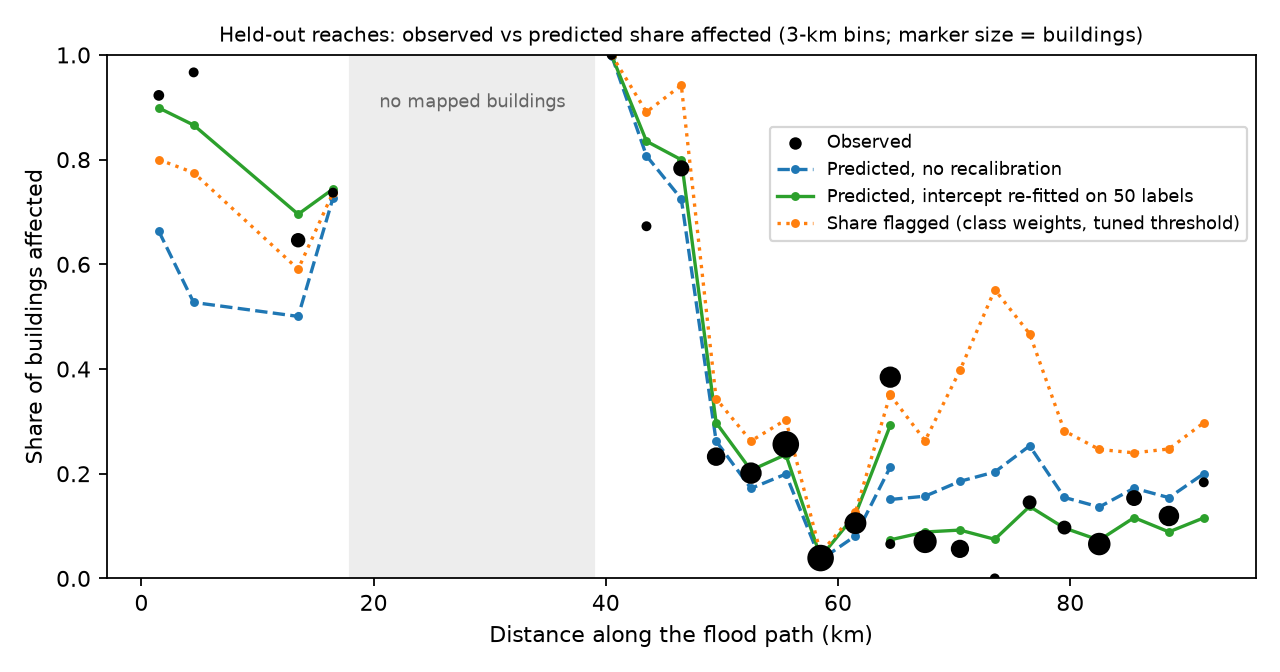
\includegraphics[width=\columnwidth]{figures/fig_damaged_share.png}
  \caption{Observed and predicted share of affected buildings per 3-km bin of the held-out reaches (bins with at least 30 buildings; marker size shows the number of buildings).}
  \label{fig:share}
\end{figure}

\subsection{Class imbalance}
No strategy changes the ranking (Table~\ref{tab:imb}). Without correction, a 0.5 threshold misses many damaged buildings (recall 0.79 for affected); class weights, SMOTE and a tuned threshold give almost the same balanced accuracy (0.90--0.91). ISMOTE is worse for logistic regression on every measure (AUC 0.939, balanced accuracy 0.856, Brier 0.140). For random forest it matches SMOTE on affected (0.923) and is better on destroyed (AUC 0.938 vs.\ 0.924), but still below class-weighted logistic regression (0.964).

\begin{table}[t]
\centering\footnotesize
\setlength{\tabcolsep}{3pt}
\caption{Imbalance strategies, logistic regression, affected, main set (mean over held-out reaches; threshold 0.5).}\label{tab:imb}
\begin{tabular}{@{}lcccc@{}}
\toprule
\textbf{Strategy} & \textbf{AUC} & \textbf{Bal.\ acc.} & \textbf{F1} & \textbf{Brier}\\
\midrule
None & \textbf{0.971} & 0.879 & 0.776 & 0.089\\
Class weights & 0.970 & \textbf{0.910} & \textbf{0.777} & \textbf{0.078}\\
SMOTE & 0.970 & 0.907 & 0.776 & 0.081\\
ISMOTE & 0.939 & 0.856 & 0.667 & 0.140\\
\bottomrule
\end{tabular}
\end{table}

\subsection{Damage regimes}
K-means on the 3,360 affected buildings gave two weak clusters (silhouette 0.27 on a random subsample of 2,500 buildings, on which Ward clustering was also run; agreement ARI = 0.73). One is an ``open valley'' regime (2,602 buildings, median HAND 18\,m, valley width about 257\,m, mostly middle and lower reaches); the other a ``steep gorge'' regime (758 buildings, median HAND 39\,m, channel slope 2.5\%, 82\% upper reach). The share destroyed is similar (74\% and 78\%), so the clusters describe the setting of damage, and severity hardly differs between them (Fig.~\ref{fig:clusters}). The silhouette keeps falling beyond two clusters (0.19 at $k = 3$, 0.15 at $k = 5$), and the Ward dendrogram splits first into the same two groups, so the structure among affected buildings is a single contrast between the gorge and the open valley; there are no further distinct damage regimes.

\begin{figure*}[t]
  \centering
  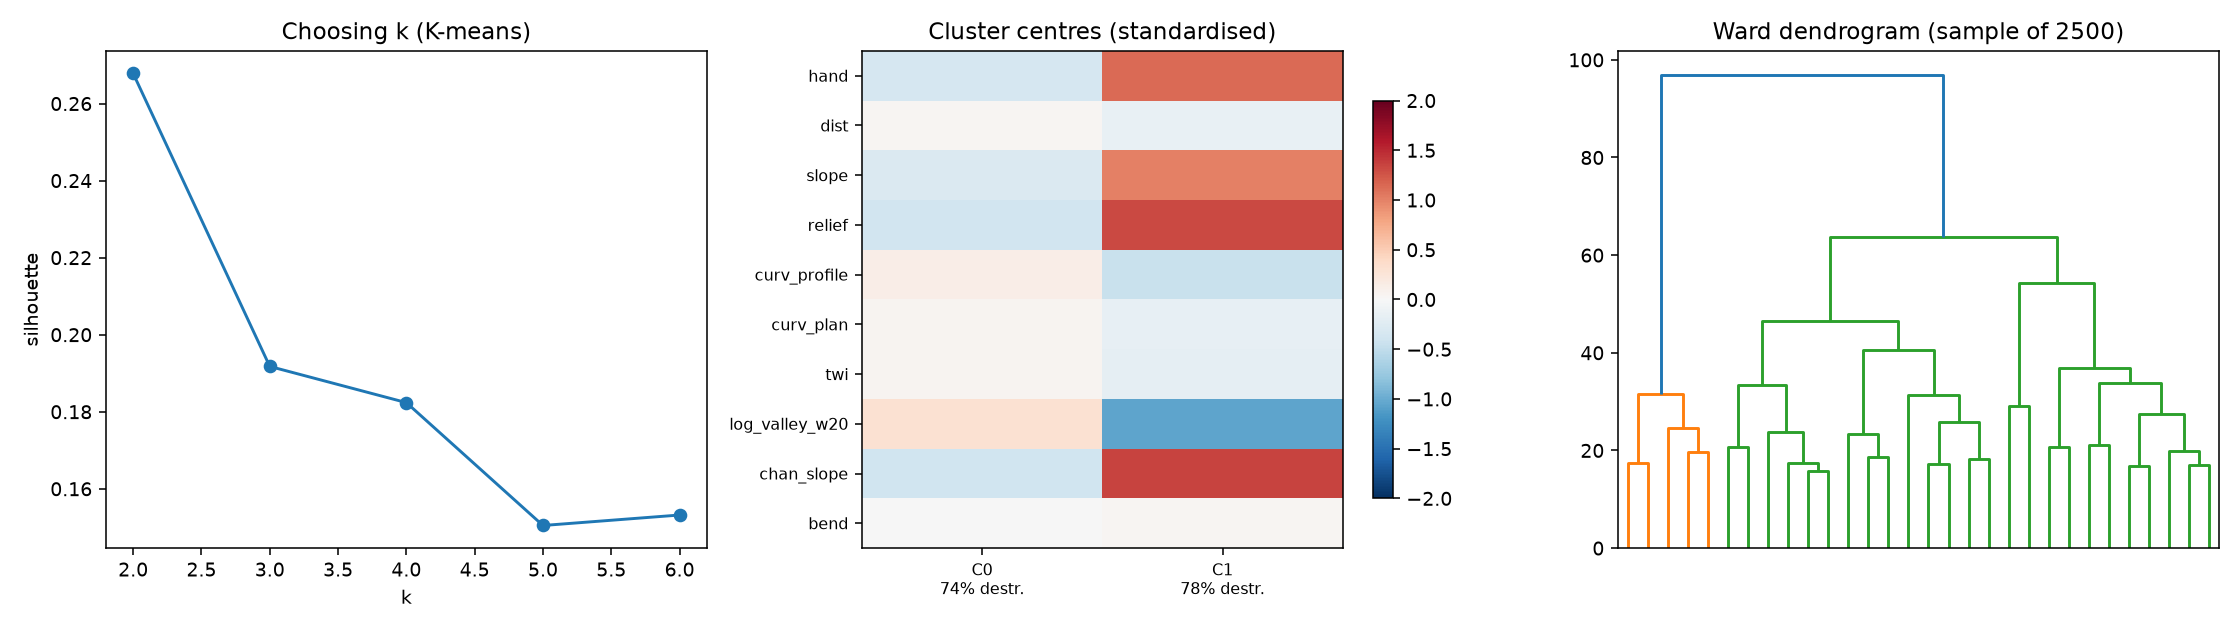
\includegraphics[width=0.92\textwidth]{figures/fig_clusters.png}
  \caption{Damage regimes among the 3,360 affected buildings. Left: silhouette by number of K-means clusters. Centre: standardised cluster centres. Right: Ward dendrogram on a sample of 2,500 buildings; its first split reproduces the two K-means clusters (ARI = 0.73).}
  \label{fig:clusters}
\end{figure*}

\subsection{Sensitivity}\label{sec:sens}
With a four-feature logistic regression (HAND, distance, slope, relief), results change little with the channel definition, the DEM and the source of the negatives (Table~\ref{tab:sens}). Measuring HAND and distance to all rivers draining at least 200, 500 or 1,000\,km$^2$ instead of to the traced flood path changes the mean affected AUC by at most 0.001, and FABDEM changes it by 0.002, although FABDEM lowers HAND by 1.5\,m on average and by more than 5\,m for 16\% of buildings. Keeping only OpenStreetMap footprints as negatives, which removes the machine-detected footprints that make Phosretar larger in our table than in the Copernicus inventory, changes affected by 0.001 and destroyed by 0.011.

\begin{table}[t]
\centering\footnotesize
\setlength{\tabcolsep}{3pt}
\caption{Sensitivity of the four-feature logistic regression (HAND, distance, slope, relief) to the terrain inputs and the negatives: mean held-out ROC-AUC over the three reaches.}\label{tab:sens}
\begin{tabular}{@{}llcc@{}}
\toprule
\textbf{DEM} & \textbf{Channel} & \textbf{Affected} & \textbf{Destroyed}\\
\midrule
GLO-30 & flood path (main) & 0.963 & 0.947\\
GLO-30 & rivers $\geq$ 200\,km$^2$ & 0.963 & 0.949\\
GLO-30 & rivers $\geq$ 500\,km$^2$ & 0.963 & 0.949\\
GLO-30 & rivers $\geq$ 1,000\,km$^2$ & 0.963 & 0.947\\
FABDEM & flood path & 0.961 & 0.946\\
FABDEM & rivers $\geq$ 500\,km$^2$ & 0.962 & 0.948\\
GLO-30 & flood path, OSM neg.\textsuperscript{a} & 0.964 & 0.936\\
\bottomrule
\end{tabular}\\[1pt]
{\scriptsize \textsuperscript{a}Only OpenStreetMap footprints kept as negatives.}
\end{table}

The label decisions were then varied for the final model (class-weighted logistic regression, main set; Table~\ref{tab:labsens}). The affected target hardly moves under any variant (0.970--0.981). The footprint-size rule R2 changes nothing. Removing the noisiest grade, \emph{possibly damaged}, raises affected and destroyed AUCs but lowers destroyed $\mid$ affected (0.833 $\rightarrow$ 0.777), because the remaining damaged class is smaller and harder to separate from destroyed. The ambiguous-row rule R1 has the largest effect. Relabelling the 1,282 R1 rows as possibly damaged drops destroyed in the upper reach to 0.657 and destroyed $\mid$ affected to near chance (0.553). Those rows lie inside the flood trace, as low as the destroyed buildings (median HAND 18\,m vs.\ 18.7\,m; 416 of them in the upper reach), so counting them as merely ``possibly damaged'' places low-lying buildings in the non-destroyed class and blurs the HAND signal. Excluding them, as in the main analysis, is therefore the conservative choice, but the destroyed results depend on it.

The audit doubt about Phosretar was tested by recoding its 275 ``destroyed'' buildings as damaged. All destroyed buildings of the lower reach are in Phosretar, so that reach can no longer be scored for the destroyed targets. In the other two reaches the destroyed AUCs change by at most 0.035 (destroyed: upper 0.952 $\rightarrow$ 0.946, middle 0.983 $\rightarrow$ 0.958; destroyed $\mid$ affected: mean 0.874 $\rightarrow$ 0.868). The doubtful Phosretar labels therefore do not drive the upstream results.

\begin{table}[t]
\centering\footnotesize
\setlength{\tabcolsep}{3pt}
\caption{Label sensitivity of the final logistic regression: mean held-out ROC-AUC over the three reaches. Aff.: affected; Destr.: destroyed; D\,$\mid$\,A: destroyed among affected.}\label{tab:labsens}
\begin{tabular}{@{}lccc@{}}
\toprule
\textbf{Variant} & \textbf{Aff.} & \textbf{Destr.} & \textbf{D\,$\mid$\,A}\\
\midrule
Main (R1--R3) & 0.970 & 0.964 & 0.833\\
R1 rows $\rightarrow$ poss.\ damaged & 0.974 & 0.845 & 0.553\\
No minimum footprint (R2 off) & 0.970 & 0.964 & 0.833\\
Minimum footprint 20\,m$^2$ & 0.971 & 0.961 & 0.833\\
Possibly damaged removed & 0.981 & 0.974 & 0.777\\
Phosretar destr.\ $\rightarrow$ damaged\textsuperscript{a} & 0.970 & 0.952 & 0.868\\
\bottomrule
\end{tabular}

{\scriptsize \textsuperscript{a}Upper and middle reaches only; the lower reach has no destroyed buildings left.}
\end{table}

\subsection{Interpretation}
\paragraph{Coefficients} HAND dominates every target (standardised coefficient for affected $-6.1$, 95\% interval $-8.6$ to $-4.7$), followed by distance to the flood path ($-1.9$). Channel slope is the third clear effect ($+1.2$; $+1.5$ for destroyed): at equal height and distance, buildings beside steeper channels were more often hit, as expected for the faster, deeper flow of the gorge. Slope ($+0.66$) and relief ($+0.50$) are positive, which means that buildings on steep terrace edges and banks were hit more often than those on the flat fan surfaces. Plan curvature is positive ($+0.31$), so at equal height and distance buildings on convex, diverging ground such as fan surfaces and spurs were hit more often than those in converging hollows. Bend exposure is significant only for destroyed ($+0.25$, interval $+0.01$ to $+0.56$): outer-bank buildings were more often destroyed but not more often affected. Valley width and the wetness index add nothing once channel slope is known. Among affected buildings, only HAND ($-3.8$) and the attenuation term ($-3.1$) separate destroyed from damaged.

\paragraph{Permutation importance on unseen reaches} Shuffling HAND lowers the held-out AUC of logistic regression by 0.37 on average; distance lowers it by 0.02, and no other feature by more than 0.007. The near-zero values of the other features do not mean they are useless: HAND and distance share much of their information, and the coefficients above show stable secondary effects \citep{molnar2022}. In the random forest with the attenuation set, the HAND $\times \log(d+10)$ interaction carries most of the importance (0.18 vs.\ 0.04 for HAND), which is the attenuation curve of Section~\ref{sec:atten} expressed as a single feature.

\paragraph{Partial dependence and rules} Both models agree on the direction of every effect (Fig.~\ref{fig:pdp}). The random forest, however, becomes flat beyond about 40\,m of HAND and 350\,m of distance, while logistic regression keeps falling. This is the extrapolation behaviour seen in the area-of-applicability analysis. The depth-3 tree gives two readable rules for \emph{affected}: (1) HAND $\leq$ 31\,m and either within 316\,m of the flood path or HAND $\leq$ 20\,m; (2) HAND $>$ 31\,m only where the channel slope exceeds 1.3\% and the building is within 241\,m of the path. The second rule is the gorge: there the flood reached higher.

\begin{figure*}[t]
  \centering
  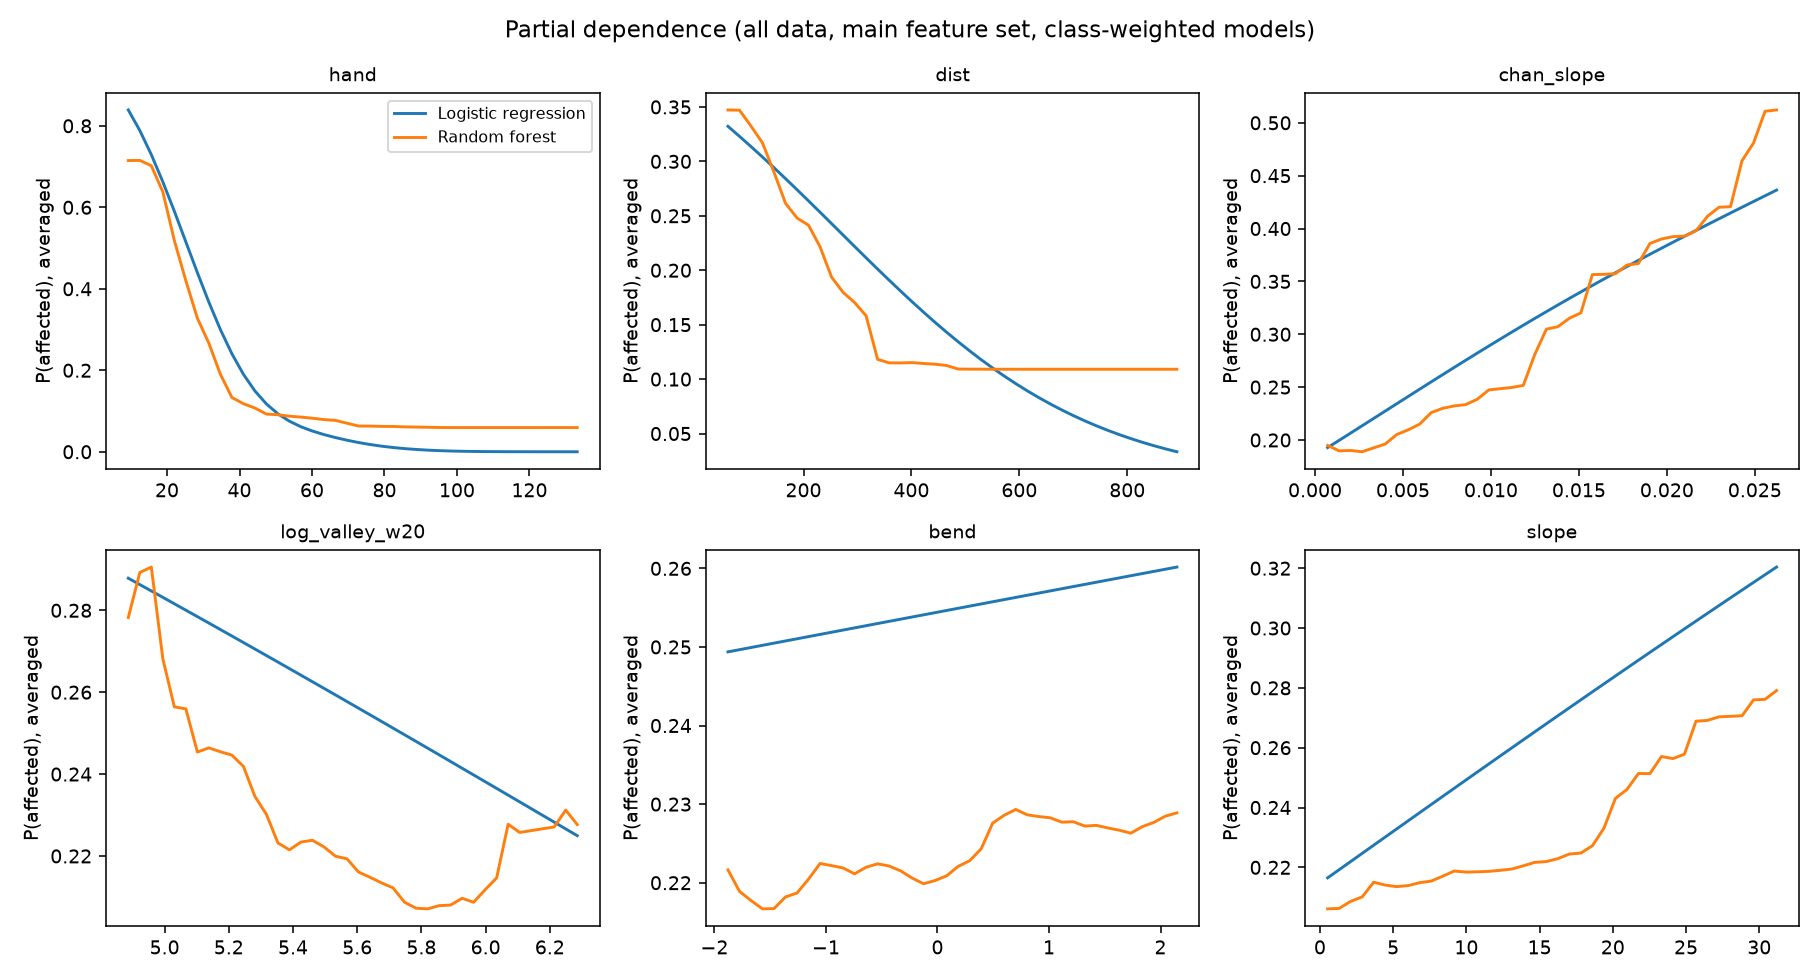
\includegraphics[width=0.92\textwidth]{figures/fig_partial_dependence.png}
  \caption{Partial dependence of the probability of being affected on six terrain features, for class-weighted logistic regression and random forest fitted on all buildings (2nd--98th percentile range of each feature).}\label{fig:pdp}
\end{figure*}

\paragraph{Where the errors are} The errors follow the calibration result (Fig.~\ref{fig:errmap}, Table~\ref{tab:conf}). In the lower reach, the threshold learned upstream predicts too much: 1,279 false positives against 10 false negatives. In the upper reach it predicts too little: 91 misses against 15 false positives, clustered in a few settlements of the gorge. The middle reach is in between (521 false positives, 143 false negatives). False positives line the river banks of the lower reach in continuous strips, which shows that the model ranks correctly along the valley but places the cut too high for the weaker flood.

\paragraph{Canopy and DEM error} Forest cover around each building was taken from ICIMOD's National Land Cover Monitoring System for 2022 \citep{nlcms} (class \emph{forest}; share within a 5 $\times$ 5 window of 30\,m pixels, about 75\,m around the building). Only 1,594 buildings (9\%) have at least 30\% forest nearby, mostly on the valley sides. Canopy does raise HAND in the surface model: relative to FABDEM, GLO-30 places buildings 1.1\,m higher where there is less than 10\% forest and 4.7\,m higher where there is more than 60\% (medians). If this bias drove the errors, damaged buildings near forest would be missed more often. They are not. Within strata of reach, HAND and distance, near-forest buildings are \emph{less} likely to be missed (Mantel--Haenszel odds ratio 0.22, $p = 0.01$) and more likely to be false positives (odds ratio 2.0, $p < 10^{-4}$). The model scores them higher because they stand on steeper ground with more relief (median slope 10.5$^\circ$ vs.\ 3.8$^\circ$ in the middle reach), which it associates with damage. ESA WorldCover (10\,m, class \emph{tree cover}) flags almost four times as many buildings as near trees but gives odds ratios in the same direction (0.53, $p = 0.003$, and 2.2, $p < 10^{-17}$). Canopy bias in the elevation model therefore does not explain the errors; the over-prediction near forest reflects the slope and relief effects instead.

\begin{figure*}[t]
  \centering
  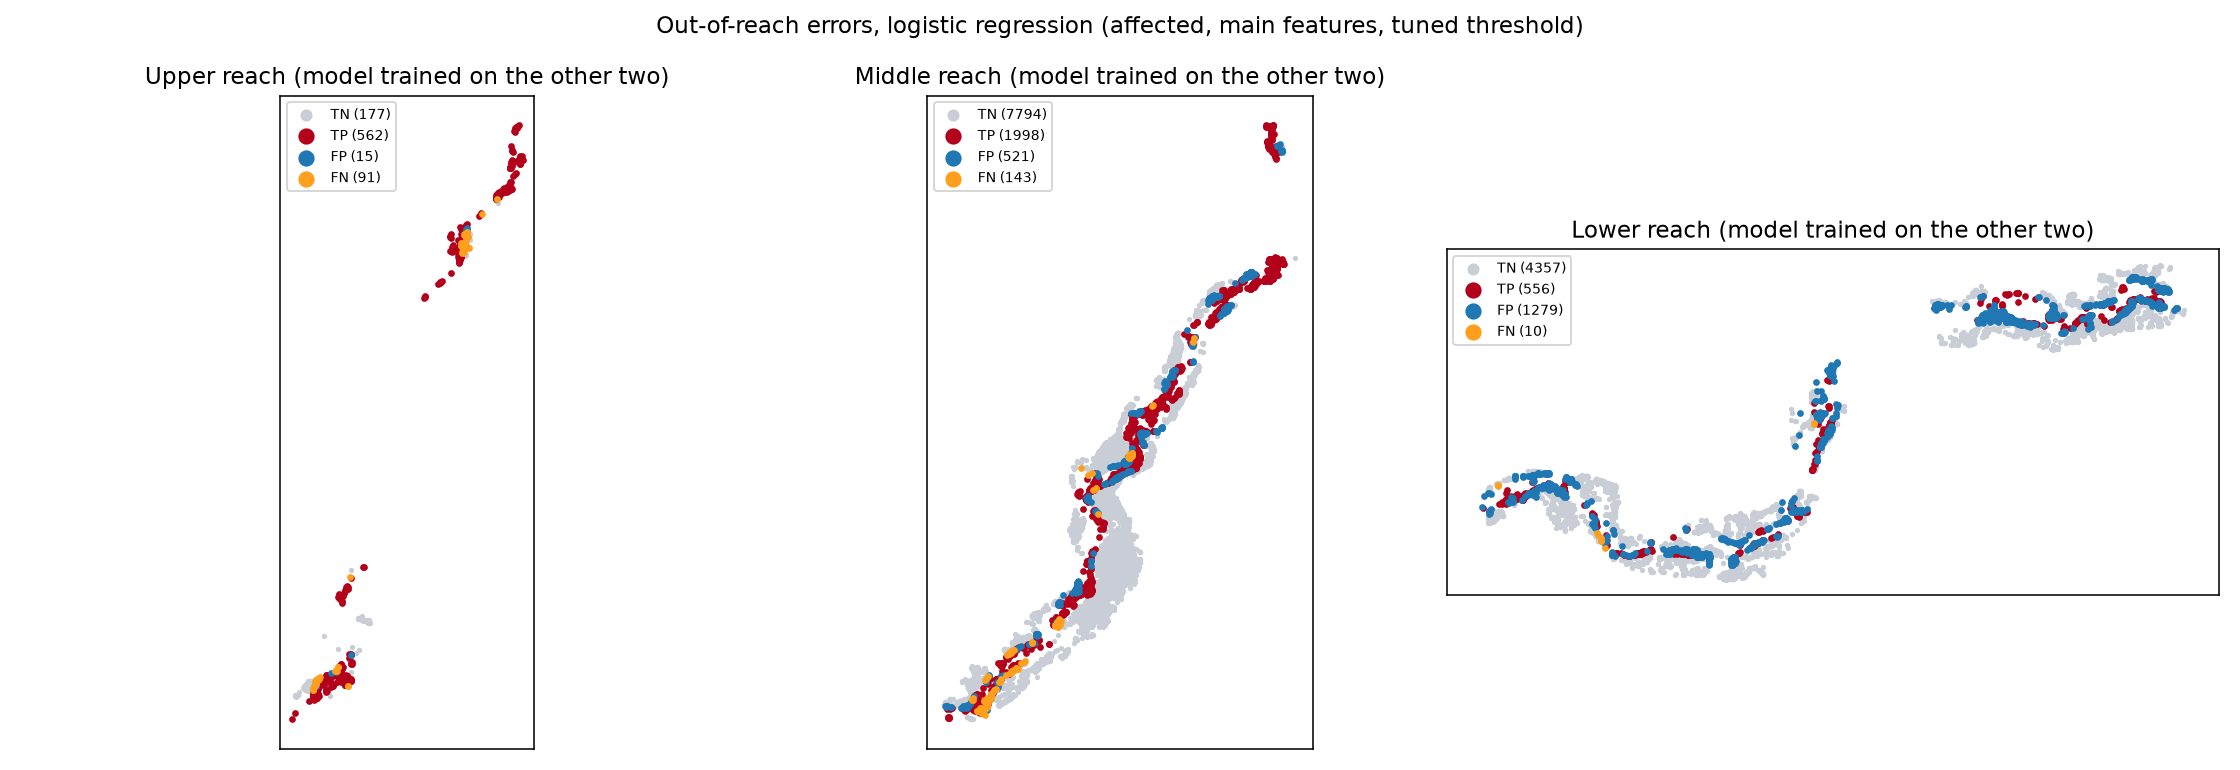
\includegraphics[width=0.92\textwidth]{figures/fig_error_map.png}
  \caption{Held-out errors of logistic regression (affected, main set, tuned threshold). Each panel shows one reach scored by a model trained on the other two. TP/TN: correct; FP: predicted affected but not; FN: affected but missed.}\label{fig:errmap}
\end{figure*}

\begin{table}[t]
\centering\footnotesize
\setlength{\tabcolsep}{4pt}
\caption{Confusion counts behind Fig.~\ref{fig:errmap}: held-out logistic regression, affected, main set, tuned threshold.}\label{tab:conf}
\begin{tabular}{@{}lrrrrrr@{}}
\toprule
\textbf{Reach} & \textbf{TP} & \textbf{FP} & \textbf{FN} & \textbf{TN} & \textbf{Recall} & \textbf{Precision}\\
\midrule
Upper & 562 & 15 & 91 & 177 & 0.86 & 0.97\\
Middle & 1,998 & 521 & 143 & 7,794 & 0.93 & 0.79\\
Lower & 556 & 1,279 & 10 & 4,357 & 0.98 & 0.30\\
\bottomrule
\end{tabular}
\end{table}

\section{Discussion}\label{sec:discussion}

\paragraph{Terrain predicts where the flood reached} Terrain alone ranks affected buildings with AUC above 0.95 in every unseen reach. Its balanced accuracy at the tuned threshold (0.91) is above the 64--72\% accuracy of structural-feature earthquake models \citep{ghimire2022,ghimire2023}, although those are three-class problems. The comparison also flatters terrain: the flood trace itself is largely controlled by terrain, so RQ1 over all buildings partly predicts flood extent. The near-channel test (AUC 0.80--0.85 for affected, 0.78--0.86 for destroyed; Table~\ref{tab:near}) and the destroyed $\mid$ affected target (0.75--0.93) show how much is left once the easy hillside buildings are removed. They are the honest measure of what terrain adds beyond ``was the building in the valley floor'', and they are the numbers we would quote for a new valley. Both are well above chance, but their intervals reach down to 0.69, and about a fifth of the ranking error remains, which is the part of damage that a 30\,m elevation model cannot see. The baselines of Table~\ref{tab:near} say where the remaining skill sits. HAND alone orders the exposed buildings as well as the full model, so the learned part is the decision threshold. A fixed HAND cut gets it badly wrong (0.64--0.68), and the attenuation and recalibration results show that it depends on the event and the reach.

\paragraph{Why linear models transfer} \citet{paulik2023} and \citet{currie2026} found that damage models lose accuracy across locations and event types. Our transfer test reproduces this for flexible models and explains it. The upper gorge lies outside the area of applicability, and tree models cannot extrapolate beyond the feature ranges they were trained on, so their predictions there flatten. A logistic regression extrapolates its monotone HAND and distance effects, which remain physically right in the gorge. Spatial cross-validation inside the training reaches cannot reveal this, even with distance-matched kNNDM folds; with only two training reaches, only a held-out reach can.

\paragraph{The flood weakens with distance} HAND$_{50}$ falls by about 20\,m per doubling of distance. The feature-group comparison suggests why the valley geometry features transfer without extrapolation: channel slope correlates with along-river distance at $\rho = -0.76$, so much of the weakening is captured by where the valley flattens and widens rather than by kilometres alone. The steep upstream part of the curve rests on only two bins, which is why the destroyed interval, whose $c = 20$\,km form leans harder on them, widens most when blocks rather than buildings are resampled (Table~\ref{tab:attboot}).

The curve can be set beside the damage thresholds of physically based studies. \citet{wang2026} found that brick--concrete buildings reach near-complete damage at a flow depth of about 2.5\,m or an impact pressure of 25\,kPa, and that momentum flux separates damage grades better than depth. In our data the destroyed curve lies below the affected curve by about 5\,m at 90\,km but by about 24\,m near the border. If depth alone set the grade, this gap would be roughly constant and of the order of a few metres. Its growth upstream suggests that in the gorge, where flow was fast and confined, the difference between damage and destruction depended on velocity and impact rather than on how deep a building was flooded. HAND is height above the river bed in a 30\,m model and is not a flow depth, so this comparison is qualitative, but it points the same way as Wang's finding on momentum flux.

\paragraph{What generalises to another flood} The calibration results answer RQ4. The ranking of buildings transfers; the probability level does not, and its error follows the attenuation curve: a model trained downstream under-predicts the stronger flood upstream, and vice versa. \citet{barnhart2024} found the same dependence on event size for physically based debris-flow forecasts. A terrain-only model can therefore be generalised in two ways. Before an event, it supplies exposure rankings or scenario maps for several HAND$_{50}$ levels. After an event, 20--50 buildings labelled from the first imagery fix the probability level. A single event-scale number, such as a gauge stage converted through HAND rating curves \citep{aristizabal2024}, could replace those labels. The affected-share comparison makes the same point in the units a responder uses: before recalibration the reach totals were off by up to 21 percentage points, after it by less than one. \citet{currie2026} likewise found that radar-based damage models lost much of their skill on events they had not seen (macro-F1 from 0.90 down to 0.41), so a large transfer error is not specific to terrain features. What is new here is that the direction of the error follows flood strength and can be corrected with a few labels.

\paragraph{What the features say about the flood} The secondary effects are small but physically consistent. They appear in the fitted coefficients and not in the held-out ranking: near the channel they do not improve on HAND alone (Table~\ref{tab:near}). Buildings beside steeper channels, on convex fan and spur surfaces and on steep terrace edges were hit more often at the same height and distance, and outer-bank buildings were more often destroyed. These are the places where a debris flood is fastest, where it spreads over the fans at tributary mouths and spills out of the channel, and where it erodes its banks. Valley width and the wetness index, which describe where water ponds slowly, add nothing. The flood thus behaved like a fast, erosive flow. Since HAND alone carries the near-channel ranking, more terrain derivatives from the same grid will not improve it. A finer elevation model, able to resolve terraces and bank edges, would sharpen HAND itself where the current model is weakest.

\paragraph{Imbalance corrections} Class weights, SMOTE and threshold tuning change the decision rule but not the ranking. This agrees with \citet{vandengoorbergh2022} and \citet{carriero2025}, who show that such corrections distort logistic-regression probabilities without improving discrimination. ISMOTE's reported gains \citep{song2024} come from 20 small benchmark sets split at random. Here it harmed logistic regression, probably because it copies the misclassified affected buildings, which in these data are the atypical or doubtful labels.

\subsection*{Limitations}
\paragraph{Labels} The damage grades come from photo-interpretation of satellite imagery, not field survey. Copernicus does not publish a per-activation accuracy for its grading products, which are produced by visual interpretation under time pressure, and in our audit the lighter grades were the least certain. In our audit 8 of the 18 judgeable Phosretar buildings graded destroyed were still standing. Undamaged buildings are inferred from the absence of a grade, so a building that the analysts missed counts as undamaged. The label sensitivity analysis shows that the affected results change little under these choices, but the destroyed results depend on how the 1,282 ambiguous rows inside the flood trace are treated.
\paragraph{Circularity} The flood trace was drawn from the same imagery and follows the terrain. Part of the skill therefore comes from predicting flood extent, and only part from predicting damage given exposure. The near-channel test (AUC 0.80--0.85) and the destroyed $\mid$ affected target (0.75--0.93) are the fairer measures of what terrain adds; the all-building scores of Table~\ref{tab:final} are an upper bound.
\paragraph{Features} Only terrain was used. Building material, storeys, age and footprint size, which drive damage in earthquake models \citep{ghimire2022,ghimire2023}, are absent, as are deposit thickness and flow velocity. The 30\,m surface model includes canopy and buildings, and HAND near forest is 1--5\,m too high, although this does not cause missed damage.
\paragraph{Design} All findings come from one event, and the three reaches are not independent samples of the cascade: the upper reach has only 845 buildings in 12 blocks, so its intervals are wide. With two training reaches, inner cross-validation cannot reproduce transfer distances, and the decision threshold learned on two reaches is applied to a third whose prevalence differs, so the thresholded metrics are less stable than the ranking metrics. The attenuation curve is an unweighted fit across bins that hold between 55 and 3,600 buildings, and its block-bootstrap interval treats 1-km blocks as independent, which is still optimistic for blocks within one settlement. ISMOTE, kNNDM and the AOA are our own re-implementations of published methods. The land-cover map has 30\,m pixels and maps forest, not individual trees around houses.

\section{Conclusions}\label{sec:conclusion}

This study asked whether terrain alone can predict building damage from the 2026 Langtang Lirung--Trishuli debris flood, and whether such a model transfers along the valley. Class-weighted logistic regression on ten DEM features ranked affected buildings with AUC 0.958--0.983 in reaches it had not seen, and with 0.80--0.85 among the near-channel buildings that the flood could actually reach, which is the fairer measure of the terrain signal; there, HAND alone ranks as well as the full model, and a fixed HAND cut does much worse (RQ1). The damaging height above the river fell by about 20\,m per doubling of distance (RQ2). Linear models transferred best; random forest and gradient boosting failed in the upstream gorge because it lies outside their area of applicability (RQ3). The ranking of buildings transferred, but the probabilities followed flood strength, and 20--50 labelled buildings were enough to recalibrate them (RQ4).

Two further results qualify these answers. Separating destroyed from damaged buildings is much harder than detecting damage (AUC 0.75--0.93) and depends on how ambiguous labels inside the flood trace are treated, so terrain says more about whether a building was reached than about how badly it was hit. And a thresholded map trained on one part of the flood overstated the affected share of the weaker lower reach threefold, although its ranking there was good; recalibrated probabilities matched the observed share in every reach to within one percentage point. The contribution of the study is therefore a split of the problem into a part that terrain can supply in advance (the ranking) and a part that must come from the event (the level).

\paragraph{Practical implications} A DEM-only model can screen exposure in other Himalayan valleys before any event. Setback heights above the river should depend on distance from likely sources. After an event, a ranking can be produced at once and recalibrated from a few labelled buildings, and buildings outside the area of applicability can be flagged for manual review.

\paragraph{Limitations} The labels are photo-interpreted and all findings come from one event. Part of the skill is predicting flood extent. Section~\ref{sec:discussion} discusses the limitations in full.

\paragraph{Future research} The model should be tested on the July 2025 Rasuwagadhi outburst flood, which struck the same terrain with a different magnitude, once building-level labels exist; on other cascades; and with an event-scale input such as gauge stage or estimated peak discharge. A finer elevation model would show whether the weak near-channel results come from the 30\,m grid, and field-checked grades in a few settlements would bound the label error that limits the destroyed target.

\paragraph{Data and code availability}
All inputs are openly licensed (Table~\ref{tab:data}); FABDEM and the Vantor imagery are for non-commercial use. The pipeline (\texttt{pilot/01}--\texttt{30}, \texttt{run\_all.sh}) rebuilds every number and figure from the raw downloads, with a pinned environment in \texttt{requirements.txt}. The code, the cleaned building table, the audit judgements and this manuscript are at \url{https://github.com/rustamniraula90/langtang-trishuli-damage} (MIT licence for code, tag v1.0.0); a DOI will be minted on acceptance.

\bibliographystyle{IEEEtranN}
\bibliography{refs}

\end{document}
